\chapter{多方策略的响应与演化}
\label{chap:game-theory-and-multi-agent-decision}

两个人共用一个房间，却分别控制一台加热器。一人增加供热，不仅改变自己的舒适程度，
也改变另一人的温度和下一步选择。第~\ref{chap:control-theory}章研究给定反馈怎样
控制状态，第~\ref{chap:decision-theory-and-dynamic-risk}章在既定环境中比较策略价值；
现在环境中还有会选择、会调整的参与者。一个人算出的最优策略依赖对方，而对方也在
作同样的计算。怎样定义这种相互依赖的选择？双方都愿意维持的策略组合是否存在，
实际调整又是否会走到那里？

回答这些问题，须分开三种对象：一局内的行动与状态、给定信息下的完整策略、
多局学习形成的策略序列。先确定策略能够依赖什么信息，才能计算其价值和允许的偏离；
排除有利偏离得到均衡条件，给出更新规则才得到动态系统。即使策略持续变化，也可以
比较整个序列与一个固定替代策略的累计表现。温度模型用于区分这几层判断，匹配硬币
用于展示随机化与循环，三张牌质询博弈则保留私人信息、完整计划和局部学习之间的联系。
合作时还要另问共同收益怎样分配，以及成员是否愿意接受分配。

\section{策略的多方行动与信息}
\label{sec:game-actions-information}

\subsection{参与者与联合行动}
\label{sec:game-joint-actions}

只写一人的行动还不足以确定房间温度或对局结果，需要把同一时刻所有人的选择放在一起。
战略式博弈用参与者、可选行动和各自收益描述这种依赖；它是一张完整的比较规则，
尚未规定各人怎样找到行动。

% Baseline B:333-341
\begin{definition}[有限战略式博弈]
\label{def:game-finite-strategic-game}
有限\(n\)人\term{战略式博弈}（strategic-form game）由参与者集合
\(N=\{1,\ldots,n\}\)、每人的有限行动集\(A_i\)和收益函数
\[
  u_i:A_1\times\cdots\times A_n\to\mathbb{R}
\]
组成，各$A_i$均非空。
\end{definition}

联合行动记为\(\bm a=(a_1,\ldots,a_n)\in\prod_i A_i\)。双人有限行动时，可以把
各人的收益列成一张表，从而得到矩阵表示。
% Baseline B:23-35
\begin{definition}[有限矩阵博弈]
\label{def:game-finite-matrix-game}
有限双人\term{矩阵博弈}（matrix game）由两组非空有限行动
\(A_1=\{1,\ldots,m\}\)、\(A_2=\{1,\ldots,n\}\)和两张收益矩阵
\(\bm{U}_1,\bm{U}_2\in\mathbb{R}^{m\times n}\)给出。第1位参与者选择行，第2位
参与者选择列，落在\((i,j)\)时，两人的收益分别为
\(\bigl((\bm{U}_1)_{i,j},(\bm{U}_2)_{i,j}\bigr)\)。若存在矩阵\(\bm{M}\)使
\(\bm{U}_1=\bm{M}\)、\(\bm{U}_2=-\bm{M}\)，双方收益之和恒为零，就得到
\term{零和博弈}（zero-sum game）。
\end{definition}
一个人增加的收益正好是另一个人的损失，因此
零和情形只需记录第1位参与者的收益矩阵\(\bm{M}\)；一般和情形则不能省略第二张矩阵。

温度与能耗通常不满足零和关系。
以下温度扩展也使用联合行动，但行动连续，不属于刚才的有限博弈定理的适用范围。

\begin{example}[两方共同加热的状态与成本]
\label{ex:game-two-heaters}
沿用温差状态\(x_t\)，把原单方加热量明确扩为两个输入之和：
\begin{equation}
  x_{t+1}=0.8x_t+u_{1,t}+u_{2,t}+w_{t+1},
  \qquad y_t=x_t+v_t.
  \label{eq:game-two-heater-dynamics}
\end{equation}
本章计算先取\(w_{t+1}=v_t=0\)。每个局内时刻，双方先观察\(x_t=y_t\)，
再同时选择各自的\(u_{i,t}\)，两项输入共同推动下一状态；本次选择不预先看到
对方的本次行动。后面的交替响应描述跨轮策略更新，不改变这项局内信息约定。默认
\(u_{i,t}\in\mathbb R\)，这是允许正负调温的无约束教学模型；若只允许加热或增加安全
约束，必须重新求解约束响应。给定局内时域\(H\)，第\(i\)方的成本可写成
\[
  J_i(\pi_1,\pi_2;x_0)
  =\sum_{t=0}^{H-1}
  \bigl[(x_{t+1}-r_i)^2+\lambda_i u_{i,t}^2\bigr],
  \qquad \lambda_i>0,
\]
其中\(\pi_i\)把本人可用历史映射为行动，\(r_i\)是舒适目标，
\(\lambda_i\)是本人能源代价权重。用于最大化的收益为\(-J_i\)，不是\(J_i\)。
\end{example}

若双方目标同为\(2\)，维持\(x_t=2\)要求总输入为\(0.4\)，并非每人都输入
\(0.4\)。对固定反馈
\(u_{i,t}=a_i-k_i(x_t-2)\)，只有\(a_1+a_2=0.4\)时，误差才满足
\[
  x_{t+1}-2=(0.8-k_1-k_2)(x_t-2).
\]
因此总增益为\(0.3\)时才复现前章的误差系数\(0.5\)。这只是给定联合反馈后的状态
计算，不证明该反馈对任一方最优。两方反馈的选择及更新须另行分析。

\subsection{纯策略与混合策略}
\label{sec:game-pure-mixed}

在匹配硬币中，双方同时选正面\(H\)或反面\(T\)，相同则第1方得\(1\)，不同则得
\(-1\)，第2方收益相反。固定选择某一面会给对方留下针对它的机会，于是需要随机化：
用一个概率分布选择行动，而不是在一局里把两个行动各执行一半。
% Baseline B:37-52
\begin{definition}[纯策略与混合策略]
\label{def:game-pure-mixed-strategy}
直接选择某一行或某一列称为\term{纯策略}（pure strategy）。在行动上选择概率分布
称为\term{混合策略}（mixed strategy）。记
\[
  \Delta_m
  =
  \left\{
    \bm{x}\in\mathbb{R}^m:
    \bm{x}\geq\bm{0},\
    \bm{1}^{\top}\bm{x}=1
  \right\}
\]
为\(m\)个行动上的概率单纯形。双方以各自的混合策略独立抽取行动。
\end{definition}

对一般有限行动集写作\(\bm\sigma_i\in\Delta(A_i)\)，联合策略为
\(\bm\sigma=(\bm\sigma_1,\ldots,\bm\sigma_n)\)，其余人的策略组合记为
\(\bm\sigma_{-i}\)。这里“联合策略”是各人的规则集合；若各人独立抽样，联合行动
服从乘积分布。如果共同装置抽取一个行动组合，再私下向各人发建议，联合分布可以相关。
两种方式即便具有同样的边缘概率，也可能产生不同收益；具体计算见
第~\ref{sec:game-payoff-relations}节。

单纯形\(\Delta_m\)嵌在\(\mathbb R^m\)中，维数为\(m-1\)，顶点对应纯行动。
匹配硬币只需一个数\(p\in[0,1]\)表示第1方选\(H\)的概率，另一个数\(q\)表示
第2方的同类概率。此时的策略空间是正方形，而不是四个纯行动组合。

\subsection{行动历史与可用信息}
\label{sec:game-extensive-information}

矩阵中的一个“行动”有时其实是一整份计划。要判断计划能否执行，需要还原每一步
发生的时间与行动者所见的信息。
% Baseline B:122-128
考虑高牌\(H\)、中牌\(M\)和低牌\(L\)。庄家从\(H\)与\(L\)中等概率发给参与者1
一张隐藏牌，\(M\)留作公共比较基准。参与者1看到自己的牌后选择质询\(B\)或放弃
\(P\)。放弃时收益为\(0\)。质询后，参与者2只知道发生了质询，不知道隐藏牌，并选择
应对\(C\)或退让\(F\)。退让时参与者1得到\(1\)；应对时，高牌使参与者1得到\(2\)，
低牌使其得到\(-2\)。参与者2得到相反收益。

这就是本章的三张牌教学任务：只随机发出高、低牌，中牌是公开比较基准，并非第三种
可能的私有牌。质询和应对发生在同一局的不同节点；学习算法在下一局改变概率，是另一个
时间尺度。
% Baseline B:797-856
\begin{definition}[有限扩展式博弈的历史树]
\label{def:game-finite-extensive-history}
\term{扩展式博弈}（extensive-form game）用历史树保留这些信息。记\(H\)为非空有限历史
集合，空历史为\(\varnothing\)。它满足前缀封闭：若一串行动属于\(H\)，删去末尾
若干行动所得的前缀仍属于\(H\)。不能再延长的历史组成终止集合\(Z\subset H\)。
若\(h\notin Z\)，可选行动集合\(A(h)\)规定合法后继\(ha\)，参与者函数\(P(h)\)
指出下一步由哪位参与者行动；机会节点记为\(P(h)=c\)，其行动概率
\(\sigma_c(a\mid h)\)已给定、非负且在\(A(h)\)上和为\(1\)。终止历史\(z\)为每位
参与者给出收益\(u_i(z)\)。对各参与者，还需指定下面的信息集划分，才能完整确定博弈。
\end{definition}

三张牌质询博弈的机会节点先选择\(H\)或\(L\)，概率各为\(1/2\)。参与者1看到牌面，
所以“拿到\(H\)”与“拿到\(L\)”属于两个不同决策位置。若他选择\(P\)，历史立即
终止；若选择\(B\)，参与者2行动。参与者2只看到“发生了质询”，无法区分历史
\((H,B)\)与\((L,B)\)。

对参与者\(i\)，记全部由其行动的非终止历史为
\[
  H_i=\{h\in H\setminus Z:P(h)=i\}.
\]
\begin{definition}[信息集]
\label{def:game-information-set}
参与者\(i\)的\term{信息集}（information set）族\(\mathcal{I}_i\)是\(H_i\)
的一个划分，每个信息集\(I\in\mathcal{I}_i\)收集参与者当时无法区分的决策历史。
同一信息集中的历史必须具有相同的合法行动集，记这个共同集合为
\(A(I)=A(h)\)，其中\(h\in I\)。
\end{definition}
否则参与者连“现在能做什么”都无法由观察确定。
牌面例子中，参与者2的信息集为
\[
  I_2=\{(H,B),(L,B)\},
\]
可选行动都是\(\{C,F\}\)。信息集不是状态的另一名称。第
~\ref{sec:decision-dynamic-programming}节中的Markov状态用于预测给定行动后的未来
分布；信息集描述当前参与者无法区分哪些历史。两个节点可以有相同物理状态，却因参与者
记得不同过去而属于不同信息集，也可以物理状态不同却因观察受限而位于同一信息集。
参与者\(i\)的纯策略必须为每个\(I\in\mathcal{I}_i\)指定一个
\(A(I)\)中的行动，包括均衡路径上不会到达的信息集；因此它是一份完整的应急计划，
而不只是实际走过路径上的动作序列。

表~\ref{tab:game-card-information}将同一个小博弈中“真实发生了什么”和“行动者
能区分什么”并列写出。参与者2在两条质询历史上必须用同一个$c$，因为他看到的数据
相同。若直接为高牌和低牌分别设置$c_H,c_L$，便改变了可用信息，得到另一个博弈，
即使收益函数没有改动也不能复用当前的均衡。

\begin{table*}[htbp]
  \centering
  \begin{tabularx}{\linewidth}{lXXX}
    \toprule
    行动者 & 真实决策历史 & 当时可区分的信息 & 合法行动规则\\
    \midrule
    参与者1 & 拿到$H$或拿到$L$ & 私人牌面可见，属于两个信息集 & 可分别选$b_H,b_L$\\
    参与者2 & $(H,B)$或$(L,B)$ & 只看到质询，属于同一信息集 & 两条历史共用应对概率$c$\\
    机会 & 初始发牌 & 已给定的环境随机化 & $P(H)=P(L)=1/2$，参与者不能选择\\
    \bottomrule
  \end{tabularx}
  \caption{三张牌教学博弈的信息约束。$b_H,b_L$为对应牌面上的质询概率，$c$为
  参与者2看到质询后的应对概率。这些行为策略记号将在下一小节正式使用。}
  \label{tab:game-card-information}
\end{table*}

参与者2不能规定“高牌质询就应对，低牌质询就退让”，因为他无法区分这两个节点。
若公开牌面，信息集就拆成两个单点集合，可实施的策略集合已经改变；不能继续使用隐藏牌
博弈的解。对零概率历史，也须预先规定行动，才能比较完整策略偏离。
但Nash条件不唯一规定零概率信息集上的信念；讨论每处的序贯理性还需额外条件。

\subsection{完整策略与行为策略}
\label{sec:game-complete-behavior}

三张牌中，第1方的完整纯计划按“高牌时行动、低牌时行动”有
\((P,P),(B,P),(P,B),(B,B)\)四种，第2方有\(F,C\)两种。
开局随机抽一份完整计划是一种实现方式；另一种是在真正到达信息集时才抽行动，
称为行为策略，也就是把随机选择写在每个可辨认的决策位置上。
% Baseline B:860-871
\begin{definition}[行为策略]
\label{def:game-behavior-strategy}
参与者\(i\)的\term{行为策略}（behavior strategy）
\(\sigma_i(a\mid I)\)在每个信息集\(I\in\mathcal{I}_i\)上分别给出$A(I)$上的概率分布；
同一信息集中的所有历史必须使用同一分布。
\end{definition}
三张牌例子可写成三个数：
\[
  b_H=\sigma_1(B\mid I_H),\qquad
  b_L=\sigma_1(B\mid I_L),\qquad
  c=\sigma_2(C\mid I_2).
\]
% Baseline B:877-944
战略式中的混合策略是在游戏开始时随机抽取一个完整纯计划；行为策略则在每个信息集
到达时随机选择。二者在一般情形下并不等价。若参与者会忘记自己早先知道的牌或采取的
行动，开局抽取的同一个随机计划可以在多个时刻制造相关性，而独立的局部随机化未必能
复制这种相关性。

\begin{definition}[完全回忆]
\label{def:game-perfect-recall}
\term{完全回忆}（perfect recall）要求参与者在同一信息集内不能混淆自己过去获得的
信息和采取的行动。更具体地说，任意两个属于同一信息集的历史，沿途经过的该参与者
信息集序列及其本人行动序列必须相同；这里的过去序列只记录当前节点之前的本人决策。
\end{definition}

\begin{theorem}[Kuhn实现等价]
\label{thm:game-kuhn-equivalence}
在有限完全回忆扩展式博弈中，对任一参与者，任意混合策略都存在一个行为策略，使二者
面对任意固定的对手与机会策略时诱导相同的终止历史分布；任意行为策略也存在具有同样
性质的混合策略。
\end{theorem}

\begin{proof}
先从混合策略构造行为策略。设\(\mu_i\)是在有限纯策略集合上的分布。完全回忆保证
每个信息集\(I\)都有唯一的本人前缀
\[
  \rho_i(I)
  =
  \bigl((I_1,a_1),\ldots,(I_k,a_k)\bigr),
\]
即到达\(I\)以前本人依次经过的信息集和采取的行动；同一\(I\)中的所有历史共享这条
前缀。记\(E_I\)为纯策略与这条前缀一致的事件。若
\(\mu_i(E_I)>0\)，定义
\[
  \sigma_i(a\mid I)
  =
  \frac{
    \mu_i\bigl(E_I\cap\{s_i:s_i(I)=a\}\bigr)
  }{
    \mu_i(E_I)
  },
\]
其中\(s_i\)表示一项完整纯策略，事件\(s_i(I)=a\)表示它在当前信息集指定行动
\(a\)；若分母为零，
就在\(A(I)\)上任取一个分布。

沿任意终止历史依次考察参与者\(i\)的行动。链式法则表明，\(\mu_i\)抽取的完整计划
与这条本人行动序列一致的概率，等于上述各条件概率的乘积，也就是行为策略
\(\sigma_i\)沿该历史贡献的到达概率。对手与机会的路径概率在两种表示下相同，所以
每个终止历史的总概率相同。分母为零的信息集只位于\(\mu_i\)赋予零概率的本人前缀
之后，任意补全都不改变这一结论。

反过来，给定行为策略\(\sigma_i\)，在游戏开始前为每个信息集独立抽取一个行动，并
把全部抽取结果组成纯策略\(s_i\)。令
\[
  \mu_i(s_i)
  =
  \prod_{I\in\mathcal{I}_i}
  \sigma_i\bigl(s_i(I)\mid I\bigr).
\]
对任意终止历史，把未出现在该历史上的信息集行动求和后都得到因子\(1\)，剩余因子
恰是行为策略沿该历史的行动概率乘积。因此该混合策略面对任意对手与机会策略，也诱导
与原行为策略相同的终止历史分布。
\end{proof}

完全回忆不能省略。考虑一位参与者先在\(I_1\)选择\(L\)或\(R\)，随后到达同一个
信息集\(I_2\)，却忘记了刚才的选择，并在\(I_2\)选择\(l\)或\(r\)。混合策略可以
各以\(1/2\)抽取完整计划\((L,l)\)与\((R,r)\)，只产生\(Ll\)和\(Rr\)两条历史。
任何行为策略若让第一步的\(L,R\)都以正概率出现，且让第二步的\(l,r\)也都以正概率
出现，就还会以正概率产生\(Lr\)和\(Rl\)；若把某个概率设为零，又无法同时保留前两条
历史各\(1/2\)的概率。因此局部独立随机化不能复现混合计划中的跨时相关性。

牌面例满足完全回忆，因为每人只行动一次。比如以概率\(2/3\)抽取\((B,P)\)、
以概率\(1/3\)抽取\((B,B)\)，等价于\(b_H=1,b_L=1/3\)的行为策略；
此处只验证表示等价，其价值及最优性将在收益计算和响应条件中分别核对。
Kuhn定理等同的是面对任意固定对手时的终局分布，不是说两种随机装置内部完全相同。

\section{策略的多方价值}
\label{sec:game-multiparty-value}

策略已经给定时，计算的是这些规则实际产生什么收益，不需要猜测参与者以后怎样改进。
有限行动表按联合概率加权，历史树按终局概率加权，两者都使用各方自己的收益。
合作分配还需先定义联盟能共同取得的价值；这个额外模型不能从一人的收益自动推出。

\subsection{给定策略下的收益计算}
\label{sec:game-fixed-policy-payoffs}

\subsubsection{联合行动下的期望收益}
\label{sec:game-joint-expected-payoff}

各人独立随机化时，联合行动\(\bm a\)的概率为\(\prod_j\sigma_j(a_j)\)，所以
% Baseline B:349-358
\begin{equation}
  u_i(\bm{\sigma})
  =
  \sum_{\bm{a}\in A_1\times\cdots\times A_n}
  \left(
    \prod_{j=1}^{n}\sigma_j(a_j)
  \right)
  u_i(\bm{a}).
  \label{eq:game-mixed-payoff-extension}
\end{equation}
后文仍用\(u_i\)表示纯行动收益及其混合延拓，参数能区分二者。双人矩阵中，
\(u_i(\bm x,\bm y)=\bm x^\top\bm U_i\bm y\)；零和时只需记录行方的收益：
% Baseline B:55-60
\begin{equation}
  u(\bm{x},\bm{y})
  =
  \bm{x}^{\top}\bm{M}\bm{y}.
  \label{eq:game-matrix-expected-payoff}
\end{equation}

若改用相关联合分布\(\mu\)，应计算
\[
  u_i(\mu)=\sum_{\bm a}\mu(\bm a)u_i(\bm a),
\]
不能把\(\mu\)擅自换成边缘概率的乘积。

匹配硬币的行方收益矩阵为
\[
  \bm M_{\mathrm{mp}}=
  \begin{pmatrix}1&-1\\-1&1\end{pmatrix}.
\]
按四个联合行动的概率加权，得到混合收益
\[
  \begin{aligned}
    u_1(p,q)&=pq+(1-p)(1-q)\\
      &\quad-p(1-q)-(1-p)q\\
      &=(2p-1)(2q-1).
  \end{aligned}
\]
给定\(q\)，纯行动\(H,T\)的收益分别为\(2q-1,1-2q\)。
例如\(p=3/4,q=1/4\)时，第1方期望收益为\(-1/4\)，第2方为\(1/4\)；
双方均匀随机时，两人的期望收益都是\(0\)。这些数是给定策略的评价，
尚未检查任何人愿不愿意改变。

\subsubsection{行动历史下的整局价值}
\label{sec:game-history-value}

历史树中，一条终局路径可能包含多次行动。要算整局收益，先把沿途概率相乘，
再按各终局收益求和。这里的路径概率与条件续局概率即使在当前不会到达的节点，
也可由策略本身计算，不必对零概率事件作除法。
% Baseline B:953-971
给定联合行为策略\(\bm{\sigma}\)，历史
\[
  h=(a_1,\ldots,a_k)
\]
的\term{到达概率}（reach probability）是沿路径各次行动概率之积。把机会也看作
固定策略，可以写成
\begin{equation}
  \pi^{\bm{\sigma}}(h)
  =
  \pi_i^{\bm{\sigma}}(h)
  \pi_{-i}^{\bm{\sigma}}(h),
  \label{eq:game-reach-factorization}
\end{equation}
其中\(\pi_i^{\bm{\sigma}}(h)\)只乘参与者\(i\)在路径上的行动概率，
\(\pi_{-i}^{\bm{\sigma}}(h)\)则乘其他参与者与机会的概率。这个分解不会声称两部分
随机变量独立；它只是把同一条路径上的乘积按行动者归组。

从历史\(h\)继续到终止历史\(z\)的条件路径概率记为
\(\pi^{\bm{\sigma}}(h,z)\)。

更明确地，若\(h_t\)是第\(t\)步前的历史，机会贡献为
\(\pi_c(h)=\prod_{t:P(h_t)=c}\sigma_c(a_t\mid h_t)\)，本人贡献为
\(\pi_i^{\bm\sigma}(h)=\prod_{t:P(h_t)=i}\sigma_i(a_t\mid I(h_t))\)；
空积为\(1\)，而\(\pi_{-i}^{\bm\sigma}(h)=\pi_c(h)\prod_{j\ne i}\pi_j^{\bm\sigma}(h)\)。
因此整局价值为
\begin{equation}
  u_i(\bm\sigma)=\sum_{z\in Z}\pi^{\bm\sigma}(z)u_i(z).
  \label{eq:game-terminal-payoff}
\end{equation}
若收益由局内阶段收益累计而来，可先对每条路径求累计收益再取期望；这与
第~\ref{sec:decision-dynamic-programming}节的续局价值使用同一求和原则，
只是现在路径概率由多方共同决定。

三张牌的六类终局概率可以直接核对：
\[
\begin{array}{c@{\quad}c@{\quad}r}
 z&\pi^{\bm\sigma}(z)&u_1(z)\\ \hline
 (H,P)&(1-b_H)/2&0\\
 (L,P)&(1-b_L)/2&0\\
 (H,B,F)&b_H(1-c)/2&1\\
 (L,B,F)&b_L(1-c)/2&1\\
 (H,B,C)&b_Hc/2&2\\
 (L,B,C)&b_Lc/2&-2
\end{array}
\]
它们的概率之和为\(1\)，从而
\begin{equation}
  u_1(b_H,b_L,c)
  =\frac12 b_H(1+c)+\frac12 b_L(1-3c),
  \qquad u_2=-u_1.
  \label{eq:game-card-behavior-payoff}
\end{equation}
例如全部取\(1/2\)时，两项分别为\(3/8\)与\(-1/8\)，整局收益为\(1/4\)。
在\((b_H,b_L,c)=(1,1/3,1/3)\)下，整局收益为\(2/3\)，发生质询的概率为
\((b_H+b_L)/2=2/3\)。给定已经质询，Bayes公式给出高、低牌概率为\(3/4,1/4\)；
因此此条件下第2方应对或退让的收益均为\(-1\)。条件收益不是事前收益：
后者还需乘上质询概率，放弃路径则贡献零。

把第1方四个完整计划分别代入式~\eqref{eq:game-card-behavior-payoff}，
并按\(F,C\)排列列方行动，就得到同一个扩展式博弈的战略式收益矩阵：
% Baseline B:131-143
\begin{equation}
  \bm{M}
  =
  \begin{pmatrix}
    0 & 0\\
    1/2 & 1\\
    1/2 & -1\\
    1 & 0
  \end{pmatrix}.
  \label{eq:game-card-normal-form}
\end{equation}
例如，计划\((B,P)\)只在拿到高牌时质询。对方退让时，收益以一半概率为\(1\)、一半
概率为\(0\)，故矩阵元素为\(1/2\)；对方应对时，相应期望为\(1\)。

该矩阵已经对机会发牌取过期望，不能在后续矩阵运算中再乘一次\(1/2\)。
在信息集上比较局部学习信号时，还会有意去掉本人的到达概率；
第~\ref{sec:game-counterfactual-comparison}节将说明这为何不同于条件期望。

\subsection{对抗与共同收益的价值关系}
\label{sec:game-payoff-relations}

同一行动空间上可以有不同的利益关系。\term{一般和博弈}（general-sum game）
允许各人收益独立规定；共同收益模型则让所有人使用同一个收益函数。
下表固定双方行动\(L,R\)，只改变收益规则，各格均按第1方、第2方排列。
\begin{table*}[htbp]
  \centering
  \begin{tabularx}{\linewidth}{lXXXX}
    \toprule
    收益关系 & $(L,L)$ & $(L,R)$ & $(R,L)$ & $(R,R)$\\
    \midrule
    零和匹配 & $(1,-1)$ & $(-1,1)$ & $(-1,1)$ & $(1,-1)$\\
    一般和选择 & $(2,2)$ & $(0,3)$ & $(3,0)$ & $(1,1)$\\
    共同协调 & $(2,2)$ & $(0,0)$ & $(0,0)$ & $(2,2)$\\
    \bottomrule
  \end{tabularx}
  \caption{同一联合行动集合上的三种教学收益。零和行中一人的增加必伴随另一人的减少；
  一般和行同时包含共同改善与利益冲突；共同协调行的两人收益逐格相同。
  表中收益仅用于说明模型关系，不表示参与者已经选定了某种行动。}
  \label{tab:game-payoff-structures}
\end{table*}

一般和行从\((R,R)\)换成\((L,L)\)能使双方收益由\(1\)增至\(2\)，称为
Pareto改进：所有人都不变差且至少一人变好。\term{Pareto最优}（Pareto optimal）
表示在所声明的可行方案集合内，不存在这样的改进。它比较共同改变后的收益，
不是固定对方时一人的改动；下一节的均衡条件将体现这一区别。
在共同协调行，双方独立均匀抽样各得期望收益\(1\)，共同建议只抽取
\((L,L),(R,R)\)且各占一半时各得\(2\)。边缘概率相同，收益却不相同。

温度模型也需要保留这项区别。只看一步并固定当前状态\(x\)，令
\[
  J_i(u_1,u_2;x)
  =(0.8x+u_1+u_2-r_i)^2+\lambda_i u_i^2.
\]
这是例~\ref{ex:game-two-heaters}在\(H=1\)时的成本。取\(x=0,r_1=r_2=2\)、
\(\lambda_1=\lambda_2=1\)，若\((u_1,u_2)=(1,0)\)，两人成本分别为\(2,1\)。
改成\((0.8,0.8)\)时，下一时刻温差为\(1.6\)，两人成本均为
\(0.4^2+0.8^2=0.8\)。共同改善确实可能，但每人是否愿意维持该行动，
还要检查固定另一人之后的响应。

\subsection{合作价值的贡献与分配}
\label{sec:game-credit-allocation-multiparty-payoffs}

\subsubsection{联盟价值与边际贡献}
\label{sec:game-coalition-value}

若参与者决定共享信息或资源，问题转为合作能产生多少额外价值，以及如何分给成员。
这里的\term{多方信用分配}（multi-party credit allocation）指按联盟贡献确定各人
份额\(\psi_i(v)\)；预算平衡要求\(\sum_i\psi_i(v)=v(N)\)。
这与把延迟奖励传回同一参与者的不同时刻不同，后者是强化学习中的时序信用分配。
% Baseline B:1682-1703
\begin{definition}[可转移效用博弈]
\label{def:game-transferable-utility-cooperation}
\term{可转移效用合作博弈}
（transferable-utility cooperative game）由参与者集合\(N\)和联盟价值函数
\[
  v:2^N\to\mathbb{R},\qquad v(\varnothing)=0
\]
组成，$N$为非空有限集合。\(v(S)\)表示联盟\(S\)独立合作时可取得并能在成员之间转移的总收益。
\end{definition}

联盟价值不是从单个模型输出自动得到的。对牌面判断任务，可以把\(v(S)\)定义为联盟
\(S\)共享信号后，相对于无信号基线减少的最优期望损失；也可以定义为收入、正确判断数
或节省的核验成本。不同定义会产生不同分配。若参与者的收益不能用同一尺度转移，例如
一方关心隐私、另一方关心延迟，就需要非可转移效用模型，不能先相加再假装总量可任意
拆分。

参与者\(i\)加入已有联盟\(S\subseteq N\setminus\{i\}\)的边际贡献为
\[
  v(S\cup\{i\})-v(S).
\]
它依赖先到者集合\(S\)。两位牌面观察者可能各自只能提供模糊线索，合在一起却能确定
牌面；此时任何一人的“独立贡献”都不能由单独使用他的信号一次决定。

\subsubsection{基于参与顺序的贡献分配}
\label{sec:game-shapley-order}

一个人先加入时贡献小，后加入时可能因已有信息互补而贡献大。对所有加入次序一视同仁，
就得到下面的排列平均规则。
% Baseline B:1707-1788
\term{Shapley值}（Shapley value）把参与者在所有随机加入次序中的边际贡献取平均
\scite{math-shapley1953value}
\begin{definition}[Shapley值]
\label{def:game-shapley-value}
对上述可转移效用博弈、\(n=|N|\)及参与者$i\in N$，其Shapley分配为
\begin{equation}
  \phi_i(v)
  =
  \sum_{S\subseteq N\setminus\{i\}}
  \frac{|S|!(n-|S|-1)!}{n!}
  \bigl[
    v(S\cup\{i\})-v(S)
  \bigr].
  \label{eq:game-shapley-value}
\end{equation}
\end{definition}
系数是随机排列中恰好由\(S\)排在\(i\)之前的概率：\(S\)内部有\(|S|!\)种次序，
其余参与者在\(i\)之后有\((n-|S|-1)!\)种次序，总排列数为\(n!\)。

Shapley值满足四项要求。若两位参与者对所有不含二者的联盟产生相同边际贡献，
\term{对称性}要求二者分配相同；若参与者对任意联盟的边际贡献都为零，
\term{虚设参与者性质}要求其分配为零；\term{有效性}要求
\(\sum_i\phi_i(v)=v(N)\)；\term{可加性}要求对两个价值函数
\(v,w\)，有\(\phi_i(v+w)=\phi_i(v)+\phi_i(w)\)。

\begin{theorem}[Shapley值的公理刻画]
\label{thm:game-shapley-characterization}
在有限可转移效用合作博弈上，同时满足对称性、虚设参与者性质、有效性和可加性的分配
规则唯一，并由式~\eqref{eq:game-shapley-value}给出。
\end{theorem}

\begin{proof}
先验证式~\eqref{eq:game-shapley-value}满足四项性质。它是随机排列下边际贡献的期望。
每个排列中，所有参与者的边际贡献沿加入次序望远镜相加为
\[
  v(N)-v(\varnothing)=v(N),
\]
取期望得到有效性。交换两位对称参与者不会改变排列分布或边际贡献分布，得到对称性。
虚设参与者的每项边际贡献都为零。边际贡献关于价值函数线性，取期望后得到可加性。

再证唯一性。设\(\Phi\)是任意满足四项公理的分配规则。对每个非空集合
\(T\subseteq N\)，定义一致联盟博弈
\[
  u_T(S)
  =
  \begin{cases}
    1,&T\subseteq S,\\
    0,&T\nsubseteq S.
  \end{cases}
\]
任意满足\(v(\varnothing)=0\)的价值函数都能唯一写成
\begin{equation}
  v
  =
  \sum_{\varnothing\neq T\subseteq N}
  c_Tu_T,
  \qquad
  c_T
  =
  \sum_{R\subseteq T}
  (-1)^{|T|-|R|}v(R),
  \label{eq:game-unanimity-basis}
\end{equation}
这是子集格上的包含--排除展开。

还要处理展开式中的任意实系数，不能只由重复相加得到整数或有理数倍。对任意
\(c\in\mathbb{R}\)，在博弈\(c\,u_T\)中，\(T\)外的参与者都是虚设参与者，分配
必须为零；\(T\)内参与者彼此对称，有效性又要求他们的分配和为\(c\)，所以每人只能
得到\(c/|T|\)。这个结论直接覆盖正、负及无理的\(c\)，没有预先假设分配规则连续。

式~\eqref{eq:game-unanimity-basis}只有有限项。可加性因此给出
\[
  \Phi(v)
  =
  \sum_{\varnothing\neq T\subseteq N}
  \Phi(c_Tu_T),
\]
而每一项已经由上一段唯一确定，故任意\(v\)上的分配也唯一。特别地，对任意
\(\alpha\in\mathbb{R}\)，对\(\alpha v\)使用同一展开便得到
\(\Phi(\alpha v)=\alpha\Phi(v)\)，这补出了实齐次性。前半部分已经证明
式~\eqref{eq:game-shapley-value}满足这些公理，故它就是唯一规则。
\end{proof}
% Baseline B:1792-1834
把牌面任务扩展为三位信息提供者。参与者1观察牌背纹理，参与者2观察发牌动作，
参与者3提供一次较弱的设备校验。以“相对于无信息基线减少的期望损失”为统一收益单位，
假设教学构造的联盟价值为
\[
\begin{array}{c@{\quad}cccccccc}
  S
  &\varnothing&\{1\}&\{2\}&\{3\}
  &\{1,2\}&\{1,3\}&\{2,3\}&\{1,2,3\}\\ \hline
  v(S)
  &0&1&1&0&3&2&2&4
\end{array}
\]
这些数值只用于展示互补贡献：前两位各自有用，二者合并额外增益较大；第三位单独无用，
却能校验已有线索。

对参与者1，四类前驱联盟的贡献给出
\begin{align*}
  \phi_1(v)
  &=
  \frac13(1-0)
  +\frac16(3-1)
  +\frac16(2-0)
  +\frac13(4-2)\\
  &=\frac53.
\end{align*}
对称性给出\(\phi_2(v)=5/3\)。参与者3的分配为
\begin{align*}
  \phi_3(v)
  &=
  \frac13(0-0)
  +\frac16(2-1)
  +\frac16(2-1)
  +\frac13(4-3)\\
  &=\frac23.
\end{align*}
三者之和为\(4=v(N)\)，与有效性一致。参与者3虽然单独价值为零，却不是虚设参与者，
因为加入\(\{1\}\)、\(\{2\}\)或\(\{1,2\}\)都会增加联盟价值。只按单人表现分配会
漏掉这种互补性。

若把价值改成模型预测分数，Shapley公式仍可计算，但解释也随之改变。它分配的是所定义
价值函数相对于基线的差，不自动等于真实因果贡献。特征彼此相关时，“缺少某个特征”的
联盟输入怎样构造还需要条件分布、边缘分布或干预语义；这些选择分别回答预测归因与因果
效应问题，不能只用同一个Shapley名称消除差异。

这个计算只回答怎样按贡献分配已定义的共同价值。成员是否能另组联盟获得更多，
以及一项分配是否会被接受，属于第~\ref{sec:game-cooperative-deviation}节的偏离检验。

\section{策略的多方响应与均衡}
\label{sec:game-best-response-equilibrium}

评价一个策略组合之后，可以固定其他人，询问一人怎样改变才更好。若各人都已作出
这种响应，便没有单方改进空间。共同建议改变了偏离者掌握的信息，合作联盟改变了
允许共同偏离的人数；每种均衡都必须同时写清这两项条件。

\subsection{给定其他策略下的最佳响应}
\label{sec:game-best-response}

对手多质询、少应对，或多加热、少加热，都可能改变本人的最优选择。
\term{最佳响应}（best response）就是把对手规则当作给定条件，选择本人的最优策略。
\begin{definition}[最佳响应]
\label{def:game-best-response}
在有限战略式博弈中，给定\(\bm\sigma_{-i}\)，参与者\(i\)的最佳响应集合为
\[
  \operatorname{BR}_i(\bm\sigma_{-i})
  =\argmax_{\widetilde{\bm\sigma}_i\in\Delta(A_i)}
       u_i(\widetilde{\bm\sigma}_i,\bm\sigma_{-i}).
\]
\end{definition}
双人零和时，行方最大化\(\bm x^\top\bm M\bm y\)，列方最小化同一个式子。
一般和时则各自最大化\(\bm x^\top\bm U_i\bm y\)，不能再将另一方收益取负。
关于本人混合概率的目标是线性的，因此至少一个纯行动达到最大值。
若多个纯行动并列最优，其任意混合也最优；最佳响应通常是集合而非唯一行动。

匹配硬币中，两行收益之差为\(4q-2\)，所以
\[
 \operatorname{BR}_1(q)=
 \begin{cases}\{1\},&q>1/2,\\[1pt]
 [0,1],&q=1/2,\\[1pt]\{0\},&q<1/2.\end{cases}
 \qquad
 \operatorname{BR}_2(p)=
 \begin{cases}\{0\},&p>1/2,\\[1pt]
 [0,1],&p=1/2,\\[1pt]\{1\},&p<1/2.\end{cases}
\]
这里集合中的数是选\(H\)的概率，不是收益。若对手均匀随机，本人任意混合都是
最佳响应；这不等于双方可以同时任意混合。

图~\ref{fig:game-matching-best-responses}把两方响应放在同一概率平面。
中心横、纵整段保存了并列最优；只有两个响应集合相交，才同时满足两方条件。
\begin{figure}[htbp]
  \centering
  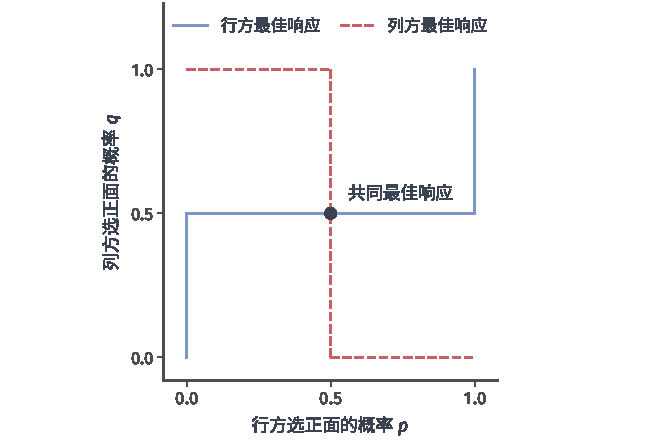
\includegraphics[width=\linewidth]{figures/01-mathematical-preliminaries/05-dynamical-systems-control-decision-and-games/matplotlib/game-matching-best-responses/figure.pdf}
  \caption{匹配硬币的最佳响应集合。横轴$p$、纵轴$q$分别是两方选$H$的概率。
  蓝色实线为行方响应，红色虚线为列方响应；在$q=1/2$处行方允许全部$p$，
  在$p=1/2$处列方允许全部$q$，唯一共同点为$(1/2,1/2)$。
  这些线段描述允许的响应，不是实际运行的学习轨迹。}
  \label{fig:game-matching-best-responses}
\end{figure}

三张牌中，固定应对概率\(c\)后，高牌质询的收益\(1+c\)总大于放弃的\(0\)，
故\(b_H=1\)是最佳选择。低牌质询收益为\(1-3c\)，所以\(c<1/3\)时选\(b_L=1\)，
\(c>1/3\)时选\(b_L=0\)，等于阈值时任意混合都可以。
反过来，由式~\eqref{eq:game-card-behavior-payoff}关于\(c\)的系数
\((b_H-3b_L)/2\)，列方在\(b_H>3b_L\)时选\(c=0\)，在\(b_H<3b_L\)时选\(c=1\)，
相等时任意\(c\)都最佳。这里比较的应对概率对两种隐藏牌必须相同，不能越过信息限制。

对温度一步成本，固定\(u_j\)后严格凸性给出唯一响应。求导并令导数为零：
\[
  \frac{\partial J_i}{\partial u_i}
  =2(0.8x+u_i+u_j-r_i)+2\lambda_i u_i=0.
\]
于是
\begin{equation}
  B_i(u_j;x)=\frac{r_i-0.8x-u_j}{1+\lambda_i}.
  \label{eq:game-heater-best-response}
\end{equation}
在\(x=0,r_i=2,\lambda_i=1\)时，对方取\(0.8\)，本人就愿意改为\(0.6\)。
即使\((0.8,0.8)\)使两人成本都低于某个其他方案，也不能据此称它为相互最佳响应。
若要求\(0\leq u_i\leq1\)，该二次成本的响应变为将右侧截到\([0,1]\)；
若还要求下一状态在\([0,3]\)，可行区间还依赖对方行动，须重新核对共同可行性。

\subsection{相互最佳响应下的Nash均衡}
\label{sec:game-nash}

\subsubsection{单方偏离与Nash条件}
\label{sec:game-nash-condition}

只求一人的响应仍没有决定联合结果。把每人的最佳响应条件同时写下，就得到
\term{Nash均衡}（Nash equilibrium）：只要其他人不变，没有谁能靠单独改策略提高收益。
\begin{definition}[Nash均衡]
\label{def:game-nash-equilibrium}
联合混合策略\(\bm\sigma^\star\)是Nash均衡，若对每个参与者\(i\)及每个可实施的
替代策略\(\widetilde{\bm\sigma}_i\)，
\begin{equation}
  u_i(\bm\sigma_i^\star,\bm\sigma_{-i}^\star)
  \geq u_i(\widetilde{\bm\sigma}_i,\bm\sigma_{-i}^\star).
  \label{eq:game-nash-no-unilateral-deviation}
\end{equation}
\end{definition}
等价地，各方最大单方改进
\(\max_{\widetilde{\bm\sigma}_i}u_i(\widetilde{\bm\sigma}_i,\bm\sigma_{-i}^\star)
-u_i(\bm\sigma^\star)\)均为零。每人都采用纯行动时称纯策略均衡，否则使用混合策略。
匹配硬币没有纯均衡：两面相同则第2方愿意改，不同则第1方愿意改；唯一混合均衡为
\(p=q=1/2\)，收益为零。

三张牌的同时响应要求\(b_H=1\)、\(b_L=1/3\)、\(c=1/3\)。
零和保证值的证书将在第~\ref{sec:game-matrix-zero-sum-duality}节独立核验。
温度一步例则解
\(2u_1+u_2=2,\ u_1+2u_2=2\)，得到唯一解
\[
  u_1^\star=u_2^\star=\frac23,\qquad x_1=\frac43,\qquad J_i^\star=\frac89.
\]
双方都不愿独改，但共同改成\((0.8,0.8)\)可把两人成本降为\(0.8<8/9\)。
事实上总成本\(2(u_1+u_2-2)^2+u_1^2+u_2^2\)严格凸，其梯度为零恰给出
\((0.8,0.8)\)。Nash条件不等于总成本最优或Pareto最优，也不比较不同均衡的公平性。
这里的\(x_1\)是从\(x_0=0\)开始的一步结果，不是闭环系统的稳态温度。

\subsubsection{响应映射与均衡存在}
\label{sec:game-equilibrium-existence}

% Baseline B:401-417
若每个最佳响应都是唯一且连续的，就可以把所有人的响应拼成映射
\[
  B(\bm{\sigma})
  =
  \bigl(
    \operatorname{BR}_1(\bm{\sigma}_{-1}),\ldots,
    \operatorname{BR}_n(\bm{\sigma}_{-n})
  \bigr),
\]
再寻找\(B(\bm{\sigma})=\bm{\sigma}\)。实际博弈常在收益并列处有多个最佳响应，
\(B\)因而不是单值连续函数。强行规定“并列时选编号最小的行动”会造成跳跃，不能直接
应用Brouwer不动点定理。

存在性论证需要两个不同层次的工具。连续单值映射先借助边界计数取得不动点；
最佳响应存在并列时，再用闭图和凸值保留整组选择。下面保留这两条工具的证明，
并在最后逐项核对有限博弈是否满足条件。
% Baseline B:420-500
\begin{lemma}[Sperner引理]
\label{lem:game-sperner}
把\(d\)维标准单纯形
\[
  \Delta^d
  =
  \left\{
    \bm{x}\in\mathbb{R}^{d+1}:
    \bm{x}\geq\bm{0},\
    \bm{1}^{\top}\bm{x}=1
  \right\}
\]
有限剖分成小单纯形。若每个剖分顶点的标签属于
\(\{0,\ldots,d\}\)，并且位于由顶点集合\(S\)张成的面上的点只能使用\(S\)中的
标签，则同时含有全部\(d+1\)种标签的小单纯形有奇数个，因而至少存在一个。
\end{lemma}

\begin{proof}
零维单纯形只有一个顶点，结论直接成立。对正维数\(d\)归纳。
\(d=1\)时，线段两个端点分别只能标\(0\)与\(1\)。沿剖分顶点
从左向右读取标签，每次改变对应一条含有两种标签的小线段；由于起点为\(0\)、终点为
\(1\)，改变次数为奇数。

先在\(d=2\)的三角形中看清高维计数。三条边上的剖分顶点只能使用相应两个端点的
标签。例如，顶点\(0\)与\(1\)之间的边只能标\(0\)或\(1\)，一维情形说明这条
边上含两种标签的小边有奇数条。计数所有带标签\(0,1\)的小边与小三角形的邻接：
内部小边被两个小三角形共享，贡献两次；大三角形边界上的小边只邻接一个小三角形，
而带齐\(0,1\)的边界小边只能出现在刚才的\(0,1\)边上。一个全标号小三角形恰有
一条\(0,1\)边，只含标签\(0,1\)且两种标签都出现的小三角形有两条这样的边，其余
小三角形没有。因此邻接总数为奇数迫使全标号小三角形的数量为奇数。一般维证明把
“小边”换成余维一的小面，把“小三角形”换成小单纯形。

假设结论对\(d-1\)维成立。在全部\(d\)维小单纯形中，计数标签集合恰为
\(\{0,\ldots,d-1\}\)的\((d-1)\)维面与小单纯形的邻接次数。内部面邻接两个
小单纯形，贡献偶数；边界面只邻接一个小单纯形。边界上只有大单纯形的
\(x_d=0\)面可能出现全部标签\(0,\ldots,d-1\)，因为其他边界面缺少其中某个允许
标签。该面继承Sperner标号，归纳假设说明其中这类小面有奇数个。因此总邻接次数为
奇数。

一个\(d\)维小单纯形若含有全部标签\(0,\ldots,d\)，恰有一个面带齐
\(0,\ldots,d-1\)，即去掉标签\(d\)顶点所得的面。若它没有标签\(d\)，却带齐
\(0,\ldots,d-1\)，则\(d+1\)个顶点中恰有一个标签重复，去掉任一重复标签顶点都会
得到这样的面，所以贡献两次；其余小单纯形贡献零次。总邻接次数的奇偶性因而等于全标号
小单纯形数目的奇偶性。前者为奇数，后者至少为一。
\end{proof}

\begin{theorem}[Brouwer不动点定理]
\label{thm:game-brouwer}
若\(K\subseteq\mathbb{R}^d\)非空、紧且凸，则每个连续映射
\(f:K\to K\)至少有一个不动点。
\end{theorem}

\begin{proof}
先令\(K=\Delta^d\)。取网格直径趋于零的一列单纯形剖分。若某个剖分顶点
\(\bm{x}\)已经满足\(f(\bm{x})=\bm{x}\)，结论成立；否则因为
\(\sum_jx_j=\sum_jf_j(\bm{x})=1\)，至少存在一个坐标\(j\)满足
\(x_j>f_j(\bm{x})\)，任选这样的\(j\)作为标签。若\(x_j=0\)，这个严格不等式
不可能成立，所以边界标号满足引理~\ref{lem:game-sperner}的条件。

每个剖分因而都有一个全标号小单纯形。对第\(k\)次剖分，记其中标签为\(j\)的顶点为
\(\bm{x}_{k,j}\)。由紧性可取子列，使\(\bm{x}_{k,0}\to\bm{x}^\star\)；小单纯形
直径趋于零，所以每个\(\bm{x}_{k,j}\)都趋于同一个\(\bm{x}^\star\)。标签定义和
连续性给出
\[
  x_j^\star\geq f_j(\bm{x}^\star),
  \qquad j=0,\ldots,d.
\]
两边坐标和都为\(1\)，故所有不等式只能同时取等号，
\(f(\bm{x}^\star)=\bm{x}^\star\)。

对一般的非空紧凸集\(K\)，取一个包含\(K\)的有限维单纯形\(S\)，并记
\(\Pi_K:S\to K\)为到闭凸集\(K\)的欧氏投影。映射
\(g=f\circ\Pi_K:S\to K\subseteq S\)连续，前一部分给出
\(\bm{x}^\star=g(\bm{x}^\star)\)。右侧属于\(K\)，所以
\(\bm{x}^\star\in K\)且\(\Pi_K(\bm{x}^\star)=\bm{x}^\star\)，进而
\(f(\bm{x}^\star)=\bm{x}^\star\)。
\end{proof}

在区间上，这个结论退化为对\(f(x)-x\)使用介值性质；高维中没有统一的“左右端点”，
Sperner引理用边界相容标号和奇偶计数补上了这一步。Brouwer只保证不动点存在，不要求
映射压缩，因此既不保证不动点唯一，也不保证反复应用\(f\)会收敛。
% Baseline B:503-533
需要的替代对象保留全部并列响应，不强制挑选其中一个。与单值连续性相应的条件，
要求附近输入的响应不能突然出现远离当前响应集合的新值。
\begin{definition}[集合值映射与上半连续性]
\label{def:game-upper-hemicontinuous-correspondence}
设$K\subseteq\mathbb R^d$非空且紧。\term{集合值映射}（correspondence）
\(F:K\rightrightarrows K\)给每个$x\in K$指定集合$F(x)\subseteq K$；本节要求各值非空。
若对每个$x\in K$及包含$F(x)$的相对开集$O\subseteq K$，都有$x$的相对邻域$U$，
使$F(z)\subseteq O$对所有$z\in U$成立，则称$F$\term{上半连续}（upper hemicontinuous）。
\end{definition}
在当前紧域、紧值的情形，一个便于使用的等价判据是闭图性质：
\[
  x_k\to x,\quad y_k\to y,\quad y_k\in F(x_k)
  \quad\Longrightarrow\quad
  y\in F(x).
\]
闭图判据适用于后面的有限博弈，因为定义域和值域都位于有限维紧集。

这个等价关系也可以直接核对。若闭图成立而上半连续失败，就有包含\(F(x)\)的
相对开集\(O\)，以及\(x_k\to x\)、\(y_k\in F(x_k)\setminus O\)。
紧性给出\(y_k\)的收敛子列，其极限仍在闭集\(K\setminus O\)，闭图却要求极限在
\(F(x)\subset O\)，矛盾。反过来，设上半连续且各值紧，若图中的点
\((x_k,y_k)\to(x,y)\)而\(y\notin F(x)\)，紧值与\(y\)的距离为正。
可取包含\(F(x)\)且与\(y\)的某邻域不交的相对开集；上半连续迫使最终的\(y_k\)
留在前者，收敛却迫使它们进入后者，再次矛盾。

例如，对手以概率\(q\)选择左列，而某参与者的两个行动收益分别为\(q\)和\(1-q\)时，
其最佳响应对应为
\[
  \operatorname{BR}(q)
  =
  \begin{cases}
    \{\text{左}\},&q>1/2,\\
    \Delta(\{\text{左},\text{右}\}),&q=1/2,\\
    \{\text{右}\},&q<1/2.
  \end{cases}
\]
在\(q=1/2\)强行挑一个行动会造成单值选择跳跃；保留整段混合策略后，对应的值仍非空、
紧且凸，并且极限不会跳出图。这正是Kakutani定理保留并列响应的方式。
% Baseline B:536-629
闭图控制极限，凸值允许在网格上混合相邻选择。二者配合，才可以把连续映射的存在工具
扩展到集合值响应，而不是对某个不连续的并列选择直接迭代。
下面使用的多值映射不动点结论源于Kakutani定理\scite{math-kakutani1941fixed}
\begin{theorem}[Kakutani不动点定理]
\label{thm:game-kakutani}
设\(K\subseteq\mathbb{R}^d\)非空、紧且凸。若
\(F:K\rightrightarrows K\)上半连续，并且每个\(F(x)\)都非空、紧且凸，
则存在\(x^\star\in K\)满足\(x^\star\in F(x^\star)\)。
\end{theorem}

下面用单纯形细分和重心插值，把集合值映射转为Brouwer定理能够处理的连续映射。

\begin{lemma}[单纯形上的连续近似选择]
\label{lem:game-approximate-selection}
在定理~\ref{thm:game-kakutani}的条件下，取一个包含\(K\)的单纯形
\(S\subseteq\mathbb{R}^d\)，并记到\(K\)的欧氏投影为
\(\Pi_K:S\to K\)。对每个\(\varepsilon>0\)，存在连续映射
\(f_\varepsilon:S\to K\)，使每个\(x\in S\)都有\(x'\in S\)及
\(y\in F(\Pi_K(x'))\)满足
\[
  \lVert x-x'\rVert_2
  +
  \lVert f_\varepsilon(x)-y\rVert_2
  <\varepsilon.
\]
\end{lemma}

\begin{proof}
对\(S\)取一列网格直径趋于零的有限单纯形细分。固定第\(k\)次细分；对每个网格顶点
\(\bm{v}\)，从非空集合\(F(\Pi_K(\bm{v}))\)中任选一点
\(\bm{y}_{\bm{v}}\)。若\(\bm{x}\)位于顶点为
\(\bm{v}_0,\ldots,\bm{v}_d\)的一个小单纯形内，把它写成重心坐标
\[
  \bm{x}
  =
  \sum_{j=0}^{d}\lambda_j\bm{v}_j,
  \qquad
  \lambda_j\geq0,\quad
  \sum_{j=0}^{d}\lambda_j=1,
\]
并定义
\[
  f_k(\bm{x})
  =
  \sum_{j=0}^{d}\lambda_j\bm{y}_{\bm{v}_j}.
\]
相邻小单纯形在公共面上使用相同的顶点值，所以这些仿射片段拼成连续映射。又因
\(K\)凸，每个\(f_k(\bm{x})\)都属于\(K\)。

在乘积空间上使用
\(\lVert(\bm{x},\bm{y})\rVert
=\lVert\bm{x}\rVert_2+\lVert\bm{y}\rVert_2\)。
下面说明网格变细时，\((\bm{x},f_k(\bm{x}))\)会一致逼近对应
\[
  \widetilde F(\bm{x})
  =
  F(\Pi_K(\bm{x}))
\]
的图。否则存在\(\varepsilon_0>0\)和点\(\bm{x}_k\in S\)，使这些点到
\(\operatorname{graph}(\widetilde F)\)的距离始终至少为\(\varepsilon_0\)。
取包含\(\bm{x}_k\)的小单纯形及其顶点
\(\bm{v}_{k,0},\ldots,\bm{v}_{k,d}\)。由\(S\)与\(K\)的紧性，可沿一个子列令
\(\bm{x}_k\to\bm{x}\)、各重心系数收敛，并令所选的
\(\bm{y}_{k,j}\in F(\Pi_K(\bm{v}_{k,j}))\)逐项收敛到\(\bm{y}_j\)。
网格直径趋于零，所以每个\(\bm{v}_{k,j}\to\bm{x}\)；投影连续和\(F\)的闭图性质
于是给出
\[
  \bm{y}_j\in F(\Pi_K(\bm{x})).
\]
值集的凸性进一步说明重心极限
\(\bm{y}=\sum_j\lambda_j\bm{y}_j\)仍属于
\(F(\Pi_K(\bm{x}))\)。另一方面，
\(f_k(\bm{x}_k)\to\bm{y}\)，这与到图的距离保持在
\(\varepsilon_0\)以上矛盾。因此充分细的网格给出所需
\(f_\varepsilon\)。
\end{proof}

\begin{proof}[定理~\ref{thm:game-kakutani}的证明]
对\(\varepsilon_k\downarrow0\)，由引理~\ref{lem:game-approximate-selection}
得到连续映射\(f_k:S\to K\subseteq S\)。Brouwer不动点定理说明存在
\(x_k\in S\)使\(x_k=f_k(x_k)\)；由于右侧属于\(K\)，每个\(x_k\)其实都在
\(K\)中。\(K\)紧，所以某个子列收敛到\(x^\star\in K\)。

近似选择性质给出\(x_k'\in S\)与
\(y_k\in F(\Pi_K(x_k'))\)，使
\(\lVert x_k-x_k'\rVert_2+\lVert x_k-y_k\rVert_2\to0\)。因此同一子列上
\(\Pi_K(x_k')\to x^\star\)且\(y_k\to x^\star\)。\(F\)具有闭图，于是
\[
  x^\star\in F(x^\star).
\]
细分和重心插值把集合值问题变成连续单值问题，Brouwer提供近似不动点，紧性提供收敛
子列，闭图性质再把极限送回\(F\)。
\end{proof}
% Baseline B:632-686
Nash的不动点论证给出有限博弈的基本存在性结果\scite{math-nash1951noncooperative}
\begin{theorem}[有限博弈存在混合Nash均衡]
\label{thm:game-nash-existence}
每个参与者和每个行动集都有限的战略式博弈至少存在一个混合策略Nash均衡。
\end{theorem}

\begin{proof}
联合混合策略空间
\[
  K=\prod_{i=1}^{n}\Delta(A_i)
\]
是有限维非空紧凸集。定义联合最佳响应对应
\[
  F(\bm{\sigma})
  =
  \prod_{i=1}^{n}
  \operatorname{BR}_i(\bm{\sigma}_{-i}).
\]
对固定\(\bm{\sigma}_{-i}\)，收益关于
\(\bm{\sigma}_i\)连续，而概率单纯形紧，所以最大值达到，
\(\operatorname{BR}_i\)非空且紧。收益关于自身混合策略线性，两个最佳响应的
凸组合仍达到同一最大值，所以最佳响应值集是凸集。

还需核对闭图。设
\(\bm{\sigma}^{(k)}\to\bm{\sigma}\)，并且
\(\bm{\tau}_i^{(k)}\to\bm{\tau}_i\)，其中
\(\bm{\tau}_i^{(k)}
\in\operatorname{BR}_i(\bm{\sigma}_{-i}^{(k)})\)。对任意固定替代策略
\(\widetilde{\bm{\sigma}}_i\)，最佳响应性质给出
\[
  u_i(\bm{\tau}_i^{(k)},\bm{\sigma}_{-i}^{(k)})
  \geq
  u_i(\widetilde{\bm{\sigma}}_i,\bm{\sigma}_{-i}^{(k)}).
\]
有限博弈的期望收益是混合概率的多线性函数，因而连续。令\(k\to\infty\)，得到
\[
  u_i(\bm{\tau}_i,\bm{\sigma}_{-i})
  \geq
  u_i(\widetilde{\bm{\sigma}}_i,\bm{\sigma}_{-i}).
\]
这对所有替代策略成立，故
\(\bm{\tau}_i\in\operatorname{BR}_i(\bm{\sigma}_{-i})\)。
每个分量都具有闭图，有限乘积\(F\)也上半连续。

定理~\ref{thm:game-kakutani}给出
\(\bm{\sigma}^\star\in F(\bm{\sigma}^\star)\)。逐分量展开正是
\(\bm{\sigma}_i^\star
\in\operatorname{BR}_i(\bm{\sigma}_{-i}^\star)\)，也就是
式~\eqref{eq:game-nash-no-unilateral-deviation}。
\end{proof}

存在性没有给出唯一性、计算效率或学习动态收敛。即便收益矩阵很小，最佳响应也可能在
多个均衡之间切换；在“石头、剪刀、布”一类循环响应中，逐轮选择当前最佳纯行动甚至
不会收敛。第~\ref{chap:mathematical-analysis}章的压缩映射同时给出唯一不动点与
迭代收敛，而Kakutani只在更弱条件下给出至少一个不动点。这两种结论服务于不同问题。

\subsection{零和对抗下的保证与均衡}
\label{sec:game-matrix-zero-sum-duality}

均衡从双方同时响应出发；零和中还可以从一方防御所有对手策略出发。
三张牌矩阵的每行最小收益依次为\(0,1/2,-1,0\)，每列最大收益均为\(1\)。
所以只用纯计划，行方至多保证\(1/2\)，列方却只能将行方收益上界压至\(1\)；
不存在纯策略鞍点。允许混合以后，两种保证是否仍有缺口？
% Baseline B:152-274
第1位参与者在不知道对方将怎样响应时，希望最大化自己能够保证的最小收益：
\[
  \underline v
  =
  \max_{\bm{x}\in\Delta_m}
  \min_{\bm{y}\in\Delta_n}
  \bm{x}^{\top}\bm{M}\bm{y}.
\]
对固定\(\bm{x}\)，第2位参与者的目标关于\(\bm{y}\)线性，所以最小值在某个纯列
达到。因此
\[
  \min_{\bm{y}\in\Delta_n}
  \bm{x}^{\top}\bm{M}\bm{y}
  =
  \min_j(\bm{M}^{\top}\bm{x})_j.
\]
类似地，第2位参与者希望把第1位参与者的最大可得收益压低到
\[
  \overline v
  =
  \min_{\bm{y}\in\Delta_n}
  \max_{\bm{x}\in\Delta_m}
  \bm{x}^{\top}\bm{M}\bm{y}
  =
  \min_{\bm{y}\in\Delta_n}\max_i(\bm{M}\bm{y})_i.
\]

对任意\(\bm{x},\bm{y}\)，都有
\[
  \min_{\widetilde{\bm{y}}}
  u(\bm{x},\widetilde{\bm{y}})
  \leq
  u(\bm{x},\bm{y})
  \leq
  \max_{\widetilde{\bm{x}}}
  u(\widetilde{\bm{x}},\bm{y}).
\]
分别对左侧取最大、右侧取最小，得到
\(\underline v\leq\overline v\)。这只是弱极小极大关系。要证明有限零和博弈中
两者相等，还需要说明双方约束恰好构成一对线性规划。

\begin{theorem}[有限零和博弈的极小极大定理]
\label{thm:game-finite-minimax}
对任意有限收益矩阵\(\bm{M}\)，有
\begin{equation}
  \max_{\bm{x}\in\Delta_m}
  \min_{\bm{y}\in\Delta_n}
  \bm{x}^{\top}\bm{M}\bm{y}
  =
  \min_{\bm{y}\in\Delta_n}
  \max_{\bm{x}\in\Delta_m}
  \bm{x}^{\top}\bm{M}\bm{y}.
  \label{eq:game-minimax-equality}
\end{equation}
共同数值称为博弈值\(v^\star\)。等式两侧的最优解分别称为双方的极小极大策略。
\end{theorem}

\begin{proof}
引入第1位参与者要保证的收益下界\(v\)。条件
\((\bm{M}^{\top}\bm{x})_j\geq v\)对每一列成立，恰好表示任何纯列都不能把收益压到
\(v\)以下。第1位参与者的问题因此是
\begin{equation}
  \begin{aligned}
    \max_{\bm{x},v}\quad&v\\
    \text{s.t.}\quad&
      \bm{M}^{\top}\bm{x}\geq v\bm{1},\\
    &\bm{1}^{\top}\bm{x}=1,\qquad
      \bm{x}\geq\bm{0}.
  \end{aligned}
  \label{eq:game-row-player-lp}
\end{equation}
它的最优值正是\(\underline v\)。为第一组不等式引入非负乘子
\(\bm{y}\geq\bm{0}\)，为概率归一化引入自由乘子\(w\)。
把最大化问题写成上界形式后，其拉格朗日函数可整理为
\[
  \mathcal{L}(\bm{x},v;\bm{y},w)
  =
  v+\bm{y}^{\top}
  (\bm{M}^{\top}\bm{x}-v\bm{1})
  +w(1-\bm{1}^{\top}\bm{x}).
\]
若对自由变量\(v\)取上确界仍为有限值，必须有
\(\bm{1}^{\top}\bm{y}=1\)。若对\(\bm{x}\geq\bm{0}\)取上确界仍为有限值，
还必须有
\[
  \bm{M}\bm{y}\leq w\bm{1}.
\]
满足这些条件时，上确界等于\(w\)。于是对偶问题为
\begin{equation}
  \begin{aligned}
    \min_{\bm{y},w}\quad&w\\
    \text{s.t.}\quad&
      \bm{M}\bm{y}\leq w\bm{1},\\
    &\bm{1}^{\top}\bm{y}=1,\qquad
      \bm{y}\geq\bm{0}.
  \end{aligned}
  \label{eq:game-column-player-lp}
\end{equation}
它要求每个纯行的收益都不超过\(w\)，所以最优值正是\(\overline v\)。两个单纯形
都非空且紧，目标连续，因此式~\eqref{eq:game-row-player-lp}与
\eqref{eq:game-column-player-lp}都有有限最优解。第
\ref{thm:opt-lp-strong-duality}号定理给出原对偶最优值相等，即
\(\underline v=\overline v=v^\star\)。
\end{proof}

这个证明不只是交换了\(\max\)与\(\min\)。概率归一化把乘子变成对方的混合策略，
逐行动收益约束把对偶可行性变成“没有纯行动能突破当前上界”。强对偶才把两种单方
证书接成同一个博弈值。

若\(\bm{x}^\star\)与\(\bm{y}^\star\)分别是两侧最优策略，则对任意
\(\bm{x}\in\Delta_m\)、\(\bm{y}\in\Delta_n\)，
\begin{equation}
  u(\bm{x},\bm{y}^\star)
  \leq
  u(\bm{x}^\star,\bm{y}^\star)
  \leq
  u(\bm{x}^\star,\bm{y}).
  \label{eq:game-zero-sum-saddle}
\end{equation}
左侧来自\(\bm{y}^\star\)把所有行收益限制在\(v^\star\)以下，右侧来自
\(\bm{x}^\star\)对所有列保证至少\(v^\star\)。这就是混合策略上的鞍点条件。
博弈值由式~\eqref{eq:game-minimax-equality}唯一确定，但达到该值的策略可以不唯一；
把“值唯一”误读成“解唯一”，会遗漏并列最优行动形成的整个最优策略集合。

下面保留同一牌面博弈的原对偶最优证书，使数值结论不依赖“双方刚好无差异”的猜测。
% Baseline B:278-322
对式~\eqref{eq:game-card-normal-form}，令第1位参与者在计划
\((B,P)\)与\((B,B)\)上分别放置概率\(2/3\)与\(1/3\)，其余计划概率为零：
\[
  \bm{x}^\star
  =
  (0,2/3,0,1/3)^{\top}.
\]
面对退让列，期望收益为
\[
  \frac23\cdot\frac12+\frac13\cdot1
  =
  \frac23;
\]
面对应对列，期望收益为
\[
  \frac23\cdot1+\frac13\cdot0
  =
  \frac23.
\]
所以\((\bm{x}^\star,2/3)\)是式~\eqref{eq:game-row-player-lp}的可行解。

再令第2位参与者以概率\(2/3\)退让、以概率\(1/3\)应对：
\[
  \bm{y}^\star=(2/3,1/3)^{\top}.
\]
四个纯计划对它的收益依次为
\[
  0,\qquad
  \frac12\cdot\frac23+1\cdot\frac13=\frac23,\qquad
  \frac12\cdot\frac23-1\cdot\frac13=0,\qquad
  \frac23.
\]
没有一行超过\(2/3\)，所以\((\bm{y}^\star,2/3)\)是
式~\eqref{eq:game-column-player-lp}的可行解。弱对偶已经足以说明两者同时最优，
博弈值为\(v^\star=2/3\)。

从牌面条件看，这个混合计划等价于：拿到高牌总是质询，拿到低牌以概率\(1/3\)质询；
参与者2面对质询时以概率\(1/3\)应对。高牌的强行动掩护了低牌的偶尔质询，低牌的
存在又使应对者不能总是退让。这个解释依赖参与者2看不到牌面；第
~\ref{sec:game-extensive-information}节已把该信息限制写进历史树。

极小极大结论依赖零和结构。若退让、应对或交易产生了双方并不相反的成本，就不能再用
一个标量博弈值同时概括双方目标。此时仍可讨论最佳响应，但稳定性必须改用一般和均衡。
对于无限或连续行动集，有限维线性规划证明也不再直接适用；交换极大与极小通常还需要
非空紧凸策略集、收益连续以及相应的凸凹结构。

鞍点条件恰是双方的Nash条件：行方不能增加收益，列方不能降低行方收益。
反过来，任一零和Nash均衡也给出这组鞍点不等式，故其收益等于同一个博弈值。
博弈值限制最坏对手下的期望保证，不表示任一局实现的收益都等于该值。

\subsection{共同建议下的偏离与均衡}
\label{sec:game-correlated-deviations}

% Baseline B:690-785
Nash均衡要求各人的随机化彼此独立。若一个公共装置先抽取联合行动
\(\bm{A}\sim\mu\)，再分别向参与者发送建议，建议之间可以相关。关键问题变成：
参与者在看到自己的建议以后，是否愿意按建议行动。

\begin{definition}[粗相关均衡与相关均衡]
\label{def:game-coarse-correlated-equilibrium}
设$\mu$为有限战略式博弈中联合行动集$\prod_i A_i$上的概率分布。
分布\(\mu\)是\term{粗相关均衡}（coarse correlated equilibrium, CCE），若对
每个参与者\(i\)和任意固定行动\(a_i'\)，
\begin{equation}
  \mathbb{E}_{\bm{A}\sim\mu}[u_i(\bm{A})]
  \geq
  \mathbb{E}_{\bm{A}\sim\mu}
  [u_i(a_i',\bm{A}_{-i})].
  \label{eq:game-cce}
\end{equation}
偏离者必须在看到建议之前承诺改用同一个固定行动。若允许他看到建议\(A_i\)后按映射
\(\phi_i(A_i)\)改动，则要求
\begin{equation}
  \mathbb{E}_{\bm{A}\sim\mu}[u_i(\bm{A})]
  \geq
  \mathbb{E}_{\bm{A}\sim\mu}
  [u_i(\phi_i(A_i),\bm{A}_{-i})]
  \label{eq:game-correlated-equilibrium}
\end{equation}
对所有映射\(\phi_i:A_i\to A_i\)成立，这定义
\term{相关均衡}（correlated equilibrium, CE）。
\end{definition}

在有限行动集上，CE条件等价于对每对\(a_i,a_i'\in A_i\)要求
\begin{equation}
  \sum_{\bm{a}_{-i}}
  \mu(a_i,\bm{a}_{-i})
  \bigl[
    u_i(a_i,\bm{a}_{-i})
    -
    u_i(a_i',\bm{a}_{-i})
  \bigr]
  \geq0.
  \label{eq:game-ce-linear-constraints}
\end{equation}
它把“收到\(a_i\)建议后改成\(a_i'\)”的条件收益比较乘上收到该建议的概率，因此
\(\mu(A_i=a_i)=0\)时无需另外定义条件概率。CCE则把求和扩到全部\(a_i\)，对应
参与者在看见建议前就承诺使用固定的\(a_i'\)。这些都是关于\(\mu\)的线性不等式，
所以有限博弈的CE与CCE集合都是凸多面体。

相关均衡排除的偏离更丰富，所以每个CE都是CCE，反向不一定成立。独立乘积分布形式的
Nash均衡又是CE的特例。这个包含关系来自允许偏离的信息和时机，而不是来自三个名称的
“强弱等级”。具体地说，固定偏离是映射偏离的特例，所以CE条件蕴含CCE条件；在Nash
乘积分布中，对手行动与自己的建议独立，而自身混合策略支持集中的每个行动都是对
\(\bm{\sigma}_{-i}\)的最佳响应，故观察建议后改用任何行动都不能提高收益。

一个二行动协调博弈可以显示相关分布与独立随机化的差别。双方都选\(L\)或都选\(R\)
时各得\(2\)，行动不同时各得\(0\)。独立地以\(1/2\)选择两项是一个混合Nash均衡，
每人期望收益为\(1\)。公共装置若以\(1/2\)推荐\((L,L)\)、以\(1/2\)推荐
\((R,R)\)，每人期望收益为\(2\)，并且看到任一建议后偏离都会把收益降为\(0\)，
所以该分布是CE。它不是两个边缘分布的乘积，但只是相对于上述独立混合均衡改善共同
收益；该博弈的两个纯Nash均衡本来也各给双方收益\(2\)，CE并不保证优于每个Nash均衡。
第~\ref{sec:game-regret-cfr}节会看到，外部遗憾自然对应CCE，内部或交换遗憾才对应CE。

矩阵博弈中的联合分布也需要与各人的边缘分布区分。
表~\ref{tab:game-independent-correlated-actions}固定刚才协调博弈的收益和每人边缘
概率：两种制度下每人都以$1/2$选择$L$，但一个制度独立抽样，另一个制度共同推荐。
收益差来自行动间的相关性，并非某个参与者改变了单独的混合概率。
图~\ref{fig:game-correlated-mass}把两种联合概率逐格显示：独立制度仍会把一半质量放在
行动不一致的格子里，共同建议则把这部分质量移到对角线。只看两个边缘分布，无法
辨认这种差别；相关均衡的偏离检验也必须使用联合分布。
\begin{figure}[htbp]
  \centering
  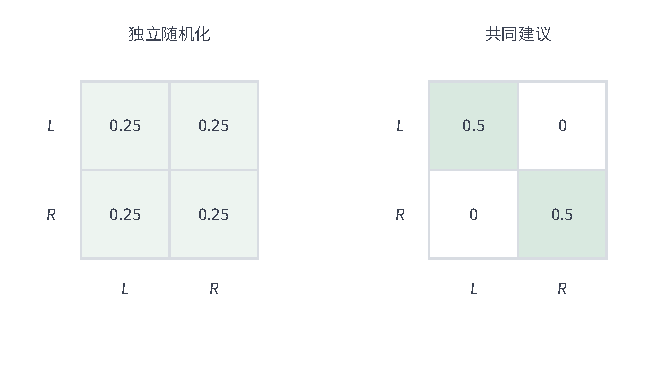
\includegraphics[width=\linewidth]{figures/01-mathematical-preliminaries/05-dynamical-systems-control-decision-and-games/tikz/game-correlated-mass/figure.pdf}
  \caption{二行动协调博弈的两个教学联合分布，共用$0$至$0.5$的概率色阶。
  行为参与者1的行动，列为参与者2的行动。左图为独立均匀策略，四格质量均为$0.25$；
  右图只推荐$(L,L)$与$(R,R)$，各占$0.5$。两者边缘概率均为$(0.5,0.5)$，
  但每人期望收益分别为$1$和$2$；相关分布并非边缘分布的乘积。}
  \label{fig:game-correlated-mass}
\end{figure}

\begin{table}[htbp]
  \centering
  \begin{tabular}{lcc}
    \toprule
    联合行动 & 独立混合概率 & 共同推荐概率\\
    \midrule
    $(L,L)$ & $1/4$ & $1/2$\\
    $(L,R)$ & $1/4$ & $0$\\
    $(R,L)$ & $1/4$ & $0$\\
    $(R,R)$ & $1/4$ & $1/2$\\
    \midrule
    每人的期望收益 & $1$ & $2$\\
    \bottomrule
  \end{tabular}
  \caption{同一边缘分布下的不同联合行动规律。教学协调博弈在相同行动时各得$2$，
  不同时各得$0$。右列是相关均衡，左列是独立混合Nash均衡；收益比较只针对这两个
  分布，纯策略协调均衡同样可以达到收益$2$。}
  \label{tab:game-independent-correlated-actions}
\end{table}

\subsection{合作分配下的偏离与稳定}
\label{sec:game-cooperative-deviation}

收益已经按贡献分配后，还须问成员愿不愿意留下来。这次允许偏离的单位可以是整个联盟，
而不只是一位参与者。这里的稳定指没有获利的退出与重组，不是策略更新对扰动的动态稳定。
% Baseline B:1838-1954
一个有效分配仍可能被某个联盟拒绝。若分配向量为\(\bm{x}\)，并满足
\[
  \sum_{i\in N}x_i=v(N),
\]
但存在联盟\(S\)使
\[
  \sum_{i\in S}x_i<v(S),
\]
那么该联盟单独合作可取得更多总收益。要求所有联盟都没有这种阻挡，并保持总收益完全
分配，得到一种对所有联盟的稳定性要求。
\begin{definition}[合作博弈的核心]
\label{def:game-cooperative-core}
对可转移效用博弈$(N,v)$，其\term{核心}（core）为分配向量$\bm x\in\mathbb R^{|N|}$的集合，
其中$\sum_{i\in N}x_i=v(N)$，并且$\sum_{i\in S}x_i\geq v(S)$对每个$S\subseteq N$成立。
\end{definition}
Shapley值不一定属于核心，核心也可能为空。
例如三人多数联盟的教学价值为$|S|\geq2$时$v(S)=1$，否则$v(S)=0$。
三人对称，Shapley值各为$1/3$；任意两人仅分到$2/3$，却能独立取得$1$，因此该分配不在核心。
更强地，三个两人联盟的不阻挡条件相加要求$2\sum_i x_i\geq3$，
有效性却要求$\sum_i x_i=1$，二者矛盾，所以核心为空。
前者由边际贡献平均和四项公理定义，后者由联盟偏离稳定性定义。

当收益不能转移时，应直接保留收益向量
\(\bm{u}(\bm{a})=(u_1(\bm{a}),\ldots,u_n(\bm{a}))\)。
第~\ref{sec:game-payoff-relations}节的Pareto条件只排除共同改进，通常形成一整个
前沿，并不选择其中哪一点。第~\ref{sec:opt-multiobjective-saddle}节中的共同下降
方向是一阶局部判据，也不能单独决定全局分配。

\begin{definition}[Nash乘积协商解]
\label{def:game-nash-bargaining-solution}
给定分歧点\(\bm{d}\in\mathbb R^n\)和可行收益集合\(U\subseteq\mathbb{R}^n\)，若下式的最大值达到，
\term{Nash协商解}（Nash bargaining solution）在参与者都不低于分歧收益的区域中
选择
\begin{equation}
  \max_{\bm{u}\in U,\ \bm{u}\geq\bm{d}}
  \prod_{i=1}^{n}(u_i-d_i),
  \label{eq:game-nash-bargaining}
\end{equation}
其中向量不等式逐坐标理解，称达到最大值的收益向量为协商解。
\end{definition}
分歧点表示谈判失败时每人的收益，因而乘积比较的是相对于
退出结果的增益，而不是原始收益本身。

\begin{theorem}[Nash乘积的存在、唯一性与Pareto性质]
\label{thm:game-nash-bargaining-properties}
设\(U\)非空、紧且凸，并存在\(\widehat{\bm{u}}\in U\)满足
\(\widehat{\bm{u}}>\bm{d}\)。则式~\eqref{eq:game-nash-bargaining}存在唯一的最优
收益向量\(\bm{u}^\star>\bm{d}\)，且\(\bm{u}^\star\)是Pareto最优的。若每位
参与者的效用与分歧收益同时作正仿射变换
\(u_i'=a_i u_i+b_i\)、\(d_i'=a_i d_i+b_i\)，其中\(a_i>0\)，变换后的解正是
\(\bm{u}^{\star\prime}=(a_i u_i^\star+b_i)_{i=1}^n\)。
\end{theorem}

\begin{proof}
个体可接受集合
\[
  K=U\cap\{\bm{u}:\bm{u}\geq\bm{d}\}
\]
非空且紧，乘积目标连续，所以最大值能够达到。严格可行点
\(\widehat{\bm{u}}\)的乘积为正，而任何至少一个坐标等于相应\(d_i\)的点乘积为
零，因此任一最优解都严格满足\(\bm{u}>\bm{d}\)。在这个正增益区域，最大化乘积
等价于最大化
\[
  F(\bm{u})=\sum_{i=1}^{n}\log(u_i-d_i).
\]
每个对数项在其坐标上严格凹，故\(F\)在正增益区域严格凹。若有两个不同最优点，凸性
保证它们的中点仍在\(U\)内，严格凹性却使中点目标严格大于两端，产生矛盾。因此最优
收益向量唯一。

若存在\(\widetilde{\bm{u}}\in U\)使
\(\widetilde{\bm{u}}\geq\bm{u}^\star\)且至少一个坐标严格更大，则所有增益保持为
正，乘积严格增加，与最优性矛盾，所以\(\bm{u}^\star\)是Pareto最优的。正仿射
变换后，每个增益变为
\(u_i'-d_i'=a_i(u_i-d_i)\)，整个乘积只乘上与候选点无关的正常数
\(\prod_i a_i\)。可行收益集合与最优点按同一坐标变换对应，因而最优选择不变。
\end{proof}

例如，两位参与者的可行收益满足
\[
  U=\{(u_1,u_2):u_1\geq0,\ u_2\geq0,\ u_1+u_2\leq6\},
  \qquad
  \bm{d}=(1,1).
\]
任何最优点都在边界\(u_1+u_2=6\)上，否则还能同时增加收益。令
\(x=u_1-1\)，则\(u_2-1=4-x\)，Nash乘积为
\[
  x(4-x)=4-(x-2)^2,
\]
故唯一解为\((u_1^\star,u_2^\star)=(3,3)\)。若只把分歧点改为\((0,1)\)，
边界上的乘积变为\(u_1(5-u_1)\)，解随之变成\((5/2,7/2)\)。这个算例说明，
协商解的“公平”相对于明确的退出收益而言，并不是脱离分歧点的绝对均分。

图~\ref{fig:game-bargaining-disagreement}将两个分歧点与对应最优收益画在同一可行
区域中。两次最优点都落在同一Pareto边界上，但分歧点改变后，乘积是在另一组增益
坐标中计算，因此最优位置也改变。唯一性来自固定可行域和固定分歧点下的严格凹目标，
不表示所有协商制度都应该选同一个收益向量。

\begin{figure*}[htbp]
  \centering
  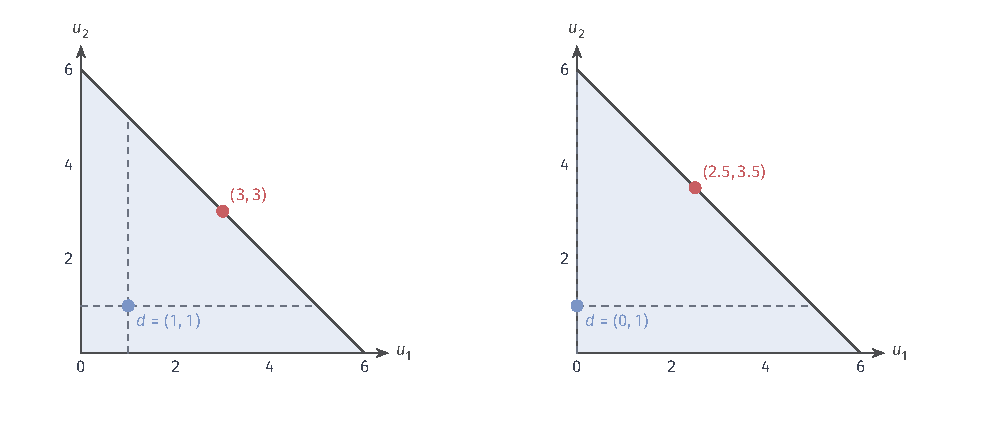
\includegraphics[width=\linewidth]{figures/01-mathematical-preliminaries/05-dynamical-systems-control-decision-and-games/tikz/game-bargaining-disagreement/figure.pdf}
  \caption{两方协商的教学可行域$u_1,u_2\geq0$、$u_1+u_2\leq6$，两图坐标一致。
  蓝点为分歧收益，红点为相对该分歧点的Nash乘积最优解。左图$\bm d=(1,1)$得到
  $(3,3)$，右图$\bm d=(0,1)$得到$(2.5,3.5)$；灰色虚线给出个体可接受的下界。
  可行总收益没有变化，变化的是退出时可得到的收益。}
  \label{fig:game-bargaining-disagreement}
\end{figure*}

没有共同严格正增益时，对数证明不适用，乘积还可能在多个零增益点同时达到最大；若
\(U\)非凸，严格凹性也不能排除不同连通部分上的多个最优点。改变分歧点会改变解，收益
若作一般非线性变换，乘积比较同样会改变。这个“协商解”与非合作博弈中的“Nash均衡”
共享提出者姓名，却解决不同问题。

至此，单方策略偏离、依建议改动和联盟退出都有了各自的比较条件。
这些条件检验一个候选结果是否会被拒绝，却没有给出参与者从初始选择走向该结果的过程。
要研究调整以后会不会回到附近、长期会不会停下来，还需要明确下一轮怎样更新。

\section{策略的多方演化与稳定}
\label{sec:game-policy-evolution}

同一个博弈可以配上不同的调整过程。双方可以同时回应上一轮，也可以轮流回应对方刚
作出的选择；可以每次求精确最优，也可以只沿当前收益增加的方向移动一小步。
这些过程共享收益函数，却不共享轨迹。因而必须先写出更新，才能讨论均衡附近的扰动
或长期极限。

\subsection{更新规则与策略序列}
\label{sec:game-update-sequences}

用\(t\)表示一局内的物理时间，用\(k=0,1,\ldots\)表示策略更新轮次。第\(k\)轮的
联合策略为\(\bm\sigma^{(k)}\)，该轮温度轨迹若需同时标明两种索引，可写成
\(x_t^{(k)}\)。本节比较相同初态、收益和信息条件下的更新；若每轮初态也变化，
就须把它纳入更新输入，不能直接套用下面的固定映射。
一般形式为
\[
  \bm\sigma^{(k+1)}
  =F_k\bigl(\bm\sigma^{(k)},\mathcal H^{(k)},\bm\xi^{(k)}\bigr),
\]
其中\(\mathcal H^{(k)}\)是更新时可用的历史信息，\(\bm\xi^{(k)}\)包括抽样或估计
噪声。即使局内策略采用随机行动，精确期望收益下的跨轮更新仍可能是确定的。
若使用累计遗憾、历史平均或动量，当前策略本身不足以决定下一步，须把这些内部量一并
放进动态系统的状态。下面先研究不显含\(k\)、无噪声的映射。

两方的同时最佳响应使用同一个旧组合：
\begin{equation}
  \sigma_1^{(k+1)}\in\operatorname{BR}_1(\sigma_2^{(k)}),
  \qquad
  \sigma_2^{(k+1)}\in\operatorname{BR}_2(\sigma_1^{(k)}).
  \label{eq:game-simultaneous-best-response}
\end{equation}
若有并列最优，这只是集合值规则，还须声明怎样选择响应。交替更新把一轮定义为两次
依次调整：
\begin{equation}
  \sigma_1^{(k+1)}\in\operatorname{BR}_1(\sigma_2^{(k)}),
  \qquad
  \sigma_2^{(k+1)}\in\operatorname{BR}_2(\sigma_1^{(k+1)}).
  \label{eq:game-alternating-best-response}
\end{equation}
第二方使用新信息，所以两式不是同一个联合映射。实际异步系统若使用延迟观测，
还要把延迟写出来。

精确响应可能代价很高。若第\(i\)方策略由
\(\bm\theta_i\in C_i\)参数化、\(C_i\)非空闭凸，且收益对该参数可微，可采用
\begin{equation}
  \bm\theta_i^{(k+1)}
  =\Pi_{C_i}\left(
    \bm\theta_i^{(k)}
    +\eta_i^{(k)}
    \nabla_{\bm\theta_i}u_i(\bm\theta^{(k)})
  \right).
  \label{eq:game-simultaneous-gradient}
\end{equation}
这是收益梯度上升；若写成本\(J_i=-u_i\)，符号改为下降。
概率单纯形上的投影保持非负与归一化，但不会自动使对方收益改善，也不保证联合映射
收缩。第~\ref{sec:game-projection-regret}节将在凸损失、梯度界和明确反馈条件下
证明它的累计保证。用估计梯度替代真梯度时，估计何时形成、是否条件无偏、方差是否
受控都是额外假设，不包含在上式的确定性分析中。

两方加热的一步模型使更新次序可以直接计算。固定\(x=0,r_1=r_2=2\)、
\(\lambda_1=\lambda_2=1\)，把每轮重新选择的一步输入写成
\(\bm u^{(k)}=(u_1^{(k)},u_2^{(k)})^\top\)，而非局内输入\(u_{i,t}\)。
由第~\ref{sec:game-best-response}节的响应公式，
\[
  B_1(u_2)=1-\frac12u_2,\qquad
  B_2(u_1)=1-\frac12u_1.
\]
同时更新从\((0,0)\)出发依次得到
\[
  (0,0),\quad (1,1),\quad (1/2,1/2),\quad(3/4,3/4),\ldots;
\]
交替更新从同一点出发，一轮结束时则依次为
\[
  (0,0),\quad(1,1/2),\quad(3/4,5/8),\quad(11/16,21/32),\ldots.
\]
两者都可能趋向\((2/3,2/3)\)，但不能凭前几个数确认收敛；下面给出误差递推。

\subsection{均衡邻域内的扰动与稳定}
\label{sec:game-local-stability}

对确定的联合映射\(F\)，先检查候选均衡\(\bm\theta^\star\)是否满足
\(F(\bm\theta^\star)=\bm\theta^\star\)。精确最佳响应若在均衡处选择当前策略，
这个条件成立；若任意打破并列最优，所选映射却可能把均衡点移走。投影梯度的不动点
只给出各方的一阶条件，只有各方收益关于自身策略凹等条件成立时，才足以推出最佳响应。
因此更新不动点与Nash均衡不能无条件等同。

在此前提下，稳定问的是初始微小偏差会不会一直小，渐近稳定还要求偏差最终趋零。
第~\ref{chap:dynamical-systems-and-state-estimation}章的定义现在应用于策略，而不是房间温度。
在内点的局部坐标中，若\(F\)连续可微，令
\(\bm e^{(k)}=\bm\theta^{(k)}-\bm\theta^\star\)，则
\[
  \bm e^{(k+1)}
  =\bm J_F(\bm\theta^\star)\bm e^{(k)}
    +o(\|\bm e^{(k)}\|).
\]
若谱半径\(\rho(\bm J_F(\bm\theta^\star))<1\)，可选一个等价向量范数，
使该矩阵的诱导范数小于\(1\)。由导数连续性，足够小邻域内的映射仍严格收缩；
取以不动点为中心的更小闭球便得到不变邻域和几何衰减。因此这是局部渐近稳定的
充分条件。若存在模大于\(1\)的特征值，光滑离散系统的线性化不稳定判据适用；
若有模等于\(1\)的特征值，一阶展开本身不作决定，须检查高阶项或其他不变量。
谱半径小于\(1\)也不要求欧氏距离每一步都下降，非正规矩阵可以先出现瞬态增长。

单纯形上的内点可先去掉一个由归一化决定的坐标，在线性切空间中应用这一判断。
边界处投影可能不可微；并列最佳响应可能发生跳变，集合值响应甚至没有普通Jacobian。
此时应直接验证距离不等式、可行方向或相应集合值条件，不能把内点判据强行套在边界上。

对加热例，令\(\bm e^{(k)}=\bm u^{(k)}-(2/3,2/3)^\top\)。同时响应恰好满足
\begin{equation}
  \bm e^{(k+1)}
  =
  \begin{pmatrix}0&-1/2\\-1/2&0\end{pmatrix}\bm e^{(k)}.
  \label{eq:game-heater-response-error}
\end{equation}
特征值为\(1/2,-1/2\)，且每轮欧氏误差恰好缩为一半。交替响应给出
\[
  \bm e^{(k+1)}
  =
  \begin{pmatrix}0&-1/2\\0&1/4\end{pmatrix}\bm e^{(k)},
\]
特征值为\(0,1/4\)。两个线性递推都对任意初值收敛，因而此处的结论不只局部成立。
它们收敛到的是固定初态的一步Nash输入，不是共同最优输入，也不意味着下一局温度
自动稳定在\(2\)。

同一成本若改用同时梯度下降，梯度向量为
\[
  \bm g(\bm u)=
  \begin{pmatrix}4u_1+2u_2-4\\2u_1+4u_2-4\end{pmatrix}.
\]
固定步长\(\eta>0\)时，误差矩阵是
\(\bm I-\eta\left(\begin{smallmatrix}4&2\\2&4\end{smallmatrix}\right)\)，
特征值为\(1-6\eta,1-2\eta\)。所以\(0<\eta<1/3\)保证全局收敛；
\(\eta=1/3\)保留一个不衰减的交替方向，更大步长会放大该方向。
即使每个人的成本关于自身行动严格凸，也不能省去步长条件。

再与式~\eqref{eq:game-two-heater-dynamics}比较。固定反馈下的状态稳定条件是
\(|0.8-k_1-k_2|<1\)，其中\(k_i\)为反馈增益；上述策略更新的条件却由响应矩阵
或梯度步长决定。一个按局内时间\(t\)判断，一个按学习轮数\(k\)判断。
若把学习与状态演化同时运行，分析对象须扩成状态与学习内部量的联合系统，本节两项
分开的计算不能替代它。

\subsection{长期更新的极限与循环}
\label{sec:game-limits-cycles}

加热例说明特定响应确实收敛，匹配硬币则说明均衡存在不足以保证这一点。
以\((p^{(k)},q^{(k)})\)表示两人选\(H\)的概率。从纯组合\((1,1)\)出发，
式~\eqref{eq:game-simultaneous-best-response}唯一地给出
\[
  (1,1)\longmapsto(1,0)\longmapsto(0,0)
  \longmapsto(0,1)\longmapsto(1,1).
\]
每一步都在最佳回应上一轮，联合序列却是四周期。若改成交替响应，则从\((1,1)\)
经一轮到\((1,0)\)，再到\((0,1)\)，此后两个组合交替，也不趋向混合均衡。
这些轨迹没有涉及并列响应点，因此循环不是由模糊的择优约定造成的。

梯度小步也不能普遍消除对抗导致的旋转。在概率正方形的内部，对收益
\(u_1=(2p-1)(2q-1)\)、\(u_2=-u_1\)同时上升，令
\(a^{(k)}=p^{(k)}-1/2\)、\(b^{(k)}=q^{(k)}-1/2\)，得到
\[
  \begin{pmatrix}a^{(k+1)}\\b^{(k+1)}\end{pmatrix}
  =
  \begin{pmatrix}1&4\eta\\-4\eta&1\end{pmatrix}
  \begin{pmatrix}a^{(k)}\\b^{(k)}\end{pmatrix}.
\]
两个特征值为\(1\pm4\eta\mathrm i\)，模为
\(\sqrt{1+16\eta^2}>1\)。在投影尚未起作用时，平方半径每轮乘上
\(1+16\eta^2\)，所以任何正的固定步长都不能使中心局部吸引。
触及边界后的轨迹还取决于投影，不能把内部递推无限延长。
若改为连续学习时间\(\tau\)的梯度流
\(\dot a=4b,\dot b=-4a\)，则
\(\frac{\mathrm d}{\mathrm d\tau}(a^2+b^2)=0\)，得到闭合圆轨道。
这里的\(\tau\)不是局内物理时间\(t\)，也不是离散轮数\(k\)。

\begin{figure*}[htbp]
  \centering
  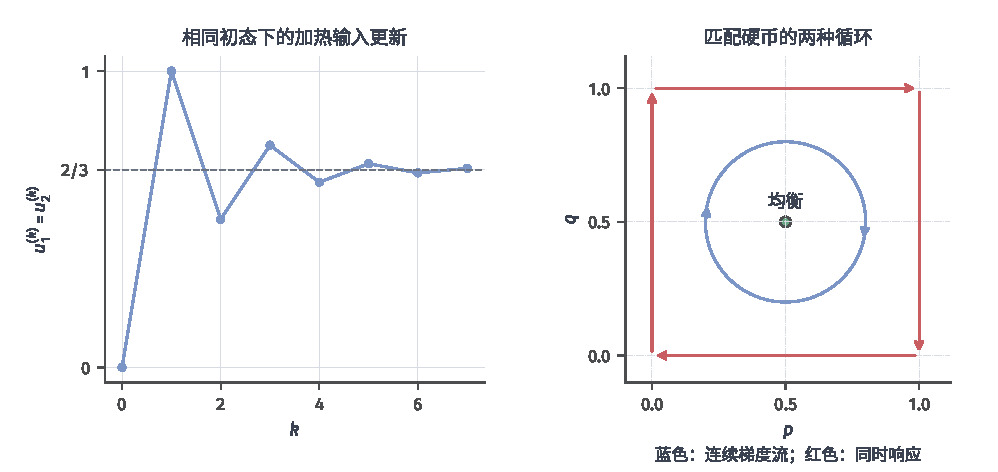
\includegraphics[width=\linewidth]{figures/01-mathematical-preliminaries/05-dynamical-systems-control-decision-and-games/matplotlib/game-update-trajectories/figure.pdf}
  \caption{两个已明确更新规则的教学轨迹。左图为相同初态下双加热器的同时最佳响应，
  从\(u_1^{(0)}=u_2^{(0)}=0\)开始，两条输入曲线重合，误差交替减半并趋向\(2/3\)。
  右图红色方形箭头是匹配硬币的离散四周期，蓝色圆是内部连续梯度流从
  \((p,q)=(0.8,0.5)\)出发的闭轨道，中心标记是Nash均衡。
  圆与方形对应不同更新，均不是最佳响应对应图中的静态集合。}
  \label{fig:game-update-trajectories}
\end{figure*}

多方演化还可以不以每个个体显式求梯度为出发点。若大量个体采用有限种行动，
收益较高的类型在下一时刻占更大比例，就得到按相对收益调整比例的
\term{复制动态}（replicator dynamics）。
在一个对称双人群体博弈中，设收益矩阵为\(\bm A\)，群体比例
\(\bm p(\tau)\in\Delta_m\)，类型\(a\)面对群体的收益为\((\bm A\bm p)_a\)，
平均收益为\(\bm p^\top\bm A\bm p\)。“对称”指交换参与者角色也交换收益，
即两方收益矩阵为\(\bm A,\bm A^\top\)，不要求\(\bm A\)本身是对称矩阵。
连续模型为
\begin{equation}
  \dot p_a
  =p_a\bigl[(\bm A\bm p)_a-\bm p^\top\bm A\bm p\bigr].
  \label{eq:game-replicator}
\end{equation}
各坐标导数之和为零，边界\(p_a=0\)上该坐标导数也为零，故单纯形保持不变。
正比例类型在静止点必须与群体平均收益相同，但未出现的类型仍可能有更高收益。
例如一个纯类型顶点总是静止点，却未必是Nash均衡；没有该类型的初始个体且没有
变异机制时，复制方程不会凭空引入它。

两方角色不同的匹配硬币应写成两个群体，而不是直接套单群体矩阵。两方复制动态为
\[
  \dot p=2p(1-p)(2q-1),\qquad
  \dot q=-2q(1-q)(2p-1).
\]
内部轨迹满足
\[
  \frac{\mathrm d}{\mathrm d\tau}
  \log\!\bigl[p(1-p)q(1-q)\bigr]=0.
\]
除中心外，每个内部水平集是围绕中心的闭曲线，向量场在其上不为零，因而形成周期运动。
这再次说明混合Nash不必吸引学习轨迹，但此处闭轨道一般不是梯度流的圆。

在对称单群体模型中，另一个问题是少量不同策略进入后能否扩张。
\begin{definition}[演化稳定策略]
\label{def:game-evolutionarily-stable}
设对称双人博弈中使用策略\(\bm p\)对阵\(\bm q\)的收益为
\(U(\bm p,\bm q)=\bm p^\top\bm A\bm q\)。
策略\(\bm p^\star\)是\term{演化稳定策略}（evolutionarily stable strategy, ESS），
若对每个\(\bm q\ne\bm p^\star\)，存在\(\bar\varepsilon(\bm q)>0\)，使所有
\(0<\varepsilon<\bar\varepsilon(\bm q)\)都满足
\[
  U(\bm p^\star,(1-\varepsilon)\bm p^\star+\varepsilon\bm q)
  >
  U(\bm q,(1-\varepsilon)\bm p^\star+\varepsilon\bm q).
\]
\end{definition}
左侧是原群体策略面对少量新策略时的收益，右侧是新策略在同一混合群体中的收益。
将两侧之差展开为
\[
  (1-\varepsilon)
  [U(\bm p^\star,\bm p^\star)-U(\bm q,\bm p^\star)]
  +\varepsilon[U(\bm p^\star,\bm q)-U(\bm q,\bm q)]
\]
可见，对每个\(\bm q\ne\bm p^\star\)，第一个括号必须为正，或在它为零时第二个
括号必须为正。这给出可直接计算的等价条件，也说明ESS必为对称Nash策略：
若第一个括号为负，再小的正入侵比例也不能满足定义。

例如\(\bm A=\left(\begin{smallmatrix}0&2\\2&0\end{smallmatrix}\right)\)，
\(\bm p^\star=(1/2,1/2)^\top\)。对任意\(\bm q=(q,1-q)^\top\)，
\[
  \begin{aligned}
    U(\bm p^\star,\bm p^\star)&=U(\bm q,\bm p^\star)=1,\\
    U(\bm p^\star,\bm q)-U(\bm q,\bm q)&=1-4q(1-q)\\
      &=(2q-1)^2.
  \end{aligned}
\]
因此\(\bm p^\star\)是ESS。此例复制动态为
\(\dot p=2p(1-p)(1-2p)\)：\(0<p<1/2\)时比例增加，\(1/2<p<1\)时减少，
所有内部初值都趋向\(1/2\)；线性化导数为\(-1\)，也证实局部吸引。
相反，两个顶点虽静止，却可被缺席类型侵入。
ESS检验少量策略入侵，动态稳定检验指定方程的扰动，Nash检验单方偏离；
这里同时成立的结论来自具体计算，不代表三种定义相同，也不涵盖有限群体随机漂移。

最后须说明“长期结果”指什么。逐轮策略是\(\bm\sigma^{(k)}\)，某个点的收敛是
\(\|\bm\sigma^{(k)}-\bm\sigma^\star\|\to0\)；接近均衡集合仅要求到该集合的距离
趋零，若集合不止一点，两者不同。有限矩阵策略的时间平均与实际行动经验分布分别为
\[
  \bar{\bm\sigma}_i^{(K)}
  =\frac1K\sum_{k=1}^K\bm\sigma_i^{(k)},\qquad
  \widehat\mu^{(K)}(\bm a)
  =\frac1K\sum_{k=1}^K\mathbb I\{\bm a^{(k)}=\bm a\}.
\]
若每轮只计算混合策略而不抽样，保留轮内独立性的对应联合平均是
\(\mu_{\mathrm{mix}}^{(K)}=K^{-1}\sum_k\bigotimes_i\bm\sigma_i^{(k)}\)，
通常不等于\(\bigotimes_i\bar{\bm\sigma}_i^{(K)}\)。
实际经验分布与这个混合分布平均之间还隔着抽样误差。
匹配硬币的四周期没有末项极限，但每满四轮，两方平均都为\((1/2,1/2)\)。
这只是该轨迹的计算结果，不能证明任意响应算法都有低遗憾。
反过来，即使已有低遗憾，也仍须说明它控制的是哪个平均对象。

\section{策略的多方累积表现}
\label{sec:game-regret-cfr}

策略没有停下来时，仍可问整个过程是否持续错过某个更好的固定选择。
遗憾把实际收益序列与同一评价序列下的替代策略比较：固定的是已经记录的对手策略，
不是假设自己改动以后对手会重新学习。若替代行为还会改变对手的后续响应，就须另建
反事实演化模型；本节基本遗憾界不比较两套重新运行的学习系统。

\subsection{固定比较策略下的累计差距}
\label{sec:game-regret-comparators}

先以损失说明符号，损失越小越好。离开当前时刻以后，回看前\(K\)轮，假设始终使用
同一个行动，它会比实际选择少付出多少损失？
\begin{definition}[外部遗憾]
\label{def:game-external-regret}
设行动集\(A\)非空且有限。同一参与者在第\(k\)轮选择\(a^{(k)}\)，面对损失函数
\(\ell^{(k)}:A\to\mathbb R\)。相对于事后最佳固定行动的
\term{外部遗憾}（external regret）为
\begin{equation}
  R_{\mathrm{ext}}^{(K)}
  =\max_{a\in A}\sum_{k=1}^K
    [\ell^{(k)}(a^{(k)})-\ell^{(k)}(a)].
  \label{eq:game-external-regret}
\end{equation}
\end{definition}
记\([z]_+=\max\{z,0\}\)。若
\([R_{\mathrm{ext}}^{(K)}]_+/K\to0\)，称该序列无外部遗憾，即平均每轮损失渐近
不高于任何固定行动。这里保留正部，是因为实际序列可能比所有固定行动都好，
使未经截断的遗憾为负；定义不要求它从负侧趋于零。
比较对象不是每轮先看到损失再重新选择的动态先知；后者通常能取得更小损失，
要对它给出累计保证，还需要变化预算或可预测性等条件。

例如两行动\(B,P\)的损失向量交替为\((0,1)\)、\((1,0)\)，共\(2m\)轮。
始终选择\(B\)的损失为\(m\)，最佳固定行动的损失也是\(m\)，外部遗憾为零；
每轮可预知损失的先知却能取得零损失，差距为\(m\)。
若每轮使用分布\(\bm w^{(k)}\)，则将实际项改为期望损失
\(\langle\bm w^{(k)},\bm\ell^{(k)}\rangle\)。
对任何固定混合分布，累计损失仍是其概率的线性函数，最小值在某个纯行动达到，
所以固定混合比较并未提高这类线性损失下的最优比较值。
但抽样行动的实际遗憾与分布的期望损失遗憾并非同一随机变量。

\begin{definition}[内部遗憾]
\label{def:game-internal-regret}
在同一行动损失序列下，\term{内部遗憾}（internal regret）允许把每次实际选择
\(a\)的轮次统一替换成另一行动\(b\)，对应差距为
\[
  R_{a\to b}^{(K)}
  =\sum_{k=1}^K\mathbb I\{a^{(k)}=a\}
    [\ell^{(k)}(a)-\ell^{(k)}(b)].
\]
对所有\((a,b)\in A\times A\)计算该量，其最大正部称为内部遗憾。
\end{definition}
控制所有这类差距，表示在知道“原本要选\(a\)”以后，也没有持续更好的统一替换。
对任意固定\(b\)，外部比较差距等于\(\sum_aR_{a\to b}^{(K)}\)；
故有限行动下无内部遗憾蕴含无外部遗憾，反向一般不成立。
这些比较分别对应相关均衡中按建议改动和粗相关均衡中的固定偏离。
改用收益\(u^{(k)}=-\ell^{(k)}\)时，遗憾写成替代收益减实际收益，正号仍表示
偏离有利，不能把两种约定混用。

\subsection{基于投影更新的累计保证}
\label{sec:game-projection-regret}

若每轮只需沿当前损失的下降方向调整，怎样控制所有轮次合起来的损失？
关键不是证明每轮都更接近当轮最优点，而是跟踪到同一个固定比较点的距离。
下面的次梯度界采用全信息或可取得真次梯度的反馈。

% Baseline B:1084-1185; learning indices normalized
第~\ref{sec:opt-projected-methods}节的投影不只用于离线优化，也能控制在线累计
损失\scite{math-zinkevich2003online}设\(C\subseteq\mathbb{R}^d\)为非空闭凸集，
直径至多为\(D\geq0\)，即对任意\(\bm{u},\bm{v}\in C\)都有
\(\lVert\bm{u}-\bm{v}\rVert_2\leq D\)。给定轮数\(K\geq1\)和步长\(\eta>0\)，
第\(k\)轮在选择
\(\bm{w}^{(k)}\in C\)后观察凸损失\(f^{(k)}\)，取次梯度
\(\bm{g}^{(k)}\in\partial f^{(k)}(\bm{w}^{(k)})\)，并假设
\(\lVert\bm{g}^{(k)}\rVert_2\leq G\)，其中\(G\geq0\)。在线投影次梯度更新为
\begin{equation}
  \bm{w}^{(k+1)}
  =
  \Pi_C\bigl(
    \bm{w}^{(k)}-\eta\bm{g}^{(k)}
  \bigr).
  \label{eq:game-online-projected-gradient}
\end{equation}

\begin{theorem}[在线投影次梯度的外部遗憾]
\label{thm:game-online-gradient-regret}
对任意比较点\(\bm{w}\in C\)，更新
\eqref{eq:game-online-projected-gradient}满足
\begin{equation}
  \sum_{k=1}^{K}
  \bigl(
    f^{(k)}(\bm{w}^{(k)})-f^{(k)}(\bm{w})
  \bigr)
  \leq
  \frac{D^2}{2\eta}
  +\frac{\eta G^2K}{2}.
  \label{eq:game-online-gradient-regret-bound}
\end{equation}
当\(D>0\)且\(G>0\)时，取\(\eta=D/(G\sqrt{K})\)，右侧为
\(DG\sqrt{K}\)。若\(D=0\)，则\(C\)只有一个点；若\(G=0\)，次梯度不等式说明
每轮差值都不大于零。两种退化情形的遗憾上界均为零，无需使用这个步长公式。
\end{theorem}

\begin{proof}
欧氏投影不会增加到任意可行点的距离，所以
\begin{align*}
  \lVert\bm{w}^{(k+1)}-\bm{w}\rVert_2^2
  &\leq
  \lVert
    \bm{w}^{(k)}-\eta\bm{g}^{(k)}-\bm{w}
  \rVert_2^2\\
  &=
  \lVert\bm{w}^{(k)}-\bm{w}\rVert_2^2
  -2\eta
  \langle
    \bm{g}^{(k)},\bm{w}^{(k)}-\bm{w}
  \rangle
  +\eta^2\lVert\bm{g}^{(k)}\rVert_2^2.
\end{align*}
凸函数的次梯度不等式给出
\[
  f^{(k)}(\bm{w}^{(k)})-f^{(k)}(\bm{w})
  \leq
  \langle
    \bm{g}^{(k)},\bm{w}^{(k)}-\bm{w}
  \rangle.
\]
把内积从距离展开式中解出并代入，得到
\[
  f^{(k)}(\bm{w}^{(k)})-f^{(k)}(\bm{w})
  \leq
  \frac{
    \lVert\bm{w}^{(k)}-\bm{w}\rVert_2^2
    -
    \lVert\bm{w}^{(k+1)}-\bm{w}\rVert_2^2
  }{2\eta}
  +\frac{\eta G^2}{2}.
\]
对\(k\)求和后，距离平方项望远镜消去，只剩初始距离上界\(D^2\)，得到
式~\eqref{eq:game-online-gradient-regret-bound}。当\(D,G>0\)时，对右侧关于
\(\eta\)配平即得\(DG\sqrt{K}\)；退化情形按定理后的说明处理。
\end{proof}

这个证明允许损失序列依赖过去行动，只要当前行动在当前损失揭晓前确定。它给出
\(O(\sqrt{K})\)累计遗憾和\(O(K^{-1/2})\)平均遗憾，却没有声称
\(\bm{w}^{(k)}\)本身收敛。把低遗憾用于博弈时，通常得到经验分布或平均策略的结论。

概率单纯形把这个通用更新接回混合策略。设行动集为
\(A=\{B,P\}\)，取\(C=\Delta(A)\)，并令第\(k\)轮两个行动的损失向量为
\(\bm{\ell}^{(k)}\)。分布\(\bm{w}\in C\)的期望损失
\[
  f^{(k)}(\bm{w})
  =
  \langle\bm{w},\bm{\ell}^{(k)}\rangle
\]
是线性函数，次梯度就是\(\bm{\ell}^{(k)}\)。若
\(\bm{w}^{(k)}=(1/2,1/2)^{\top}\)、
\(\bm{\ell}^{(k)}=(0,1)^{\top}\)且\(\eta=1/2\)，则
\[
  \Pi_{\Delta(A)}
  \left(
    \bm{w}^{(k)}-\eta\bm{\ell}^{(k)}
  \right)
  =
  (3/4,1/4)^{\top}.
\]
投影把概率从本轮损失较大的\(P\)移向\(B\)，同时保持坐标非负且和为\(1\)。
定理因而说明混合策略空间上可以构造局部无外部遗憾更新。下面的CFR在各信息集采用
遗憾匹配，而不是必须采用欧氏投影；这里的通用结果用于建立两类更新共享的无遗憾目标。

这里的\(f^{(k)}\)可由第\(k\)轮对手策略产生，损失不必跨轮相同。
固定比较点\(\bm w\)在整个求和中不变，这是望远镜论证能够直接给出外部遗憾的原因。
未知总轮数时，不能直接预设含\(K\)的固定步长；可另用递减步长或分段重启并重新累计
界。本定理只证明所声明的固定时域版本。

若只观察抽中的行动损失，通常无法直接取得完整损失向量。可构造估计量，但须声明
探索概率、条件无偏性和二阶矩界；期望界与高概率界也要分别推导。
第~\ref{chap:stochastic-processes-and-approximation}章的随机评价工具负责这些附加
误差，不可把确定性梯度界原样用于任意带噪反馈。

\subsection{基于局部遗憾的整局保证}
\label{sec:game-local-to-global-regret}

历史树的完整纯计划数可能很大，直接在它们上面运行一个更新代价高。
能否只在各信息集比较当前行动，再把局部差距合成整局保证？
信息集允许哪些偏离已在第~\ref{sec:game-extensive-information}节确定；
剩下的困难是不同位置的到达概率不同，而且改变上游策略会改变下游访问频率。

\subsubsection{信息集上的反事实收益比较}
\label{sec:game-counterfactual-comparison}

沿用第~\ref{sec:game-history-value}节的到达分解
\(\pi^{\bm\sigma}(h)=\pi_i^{\bm\sigma}(h)\pi_{-i}^{\bm\sigma}(h)\)，以及从
\(ha\)继续到终局的路径概率\(\pi^{\bm\sigma}(ha,z)\)。
若局部差距乘上当前自身到达概率，一个目前很少访问的位置几乎得不到纠正；
将来改变上游行动后，它却可能变得重要。下面暂时去掉自身前缀概率，保留对手与机会
权重，为之后比较任意完整替代策略准备可重用的局部量。

\begin{example}[同一参与者的两层决策]
\label{ex:game-two-stage-self-reach}
为单独观察自身到达权重，图~\ref{fig:game-two-stage-self-reach}给出没有对手行动和机会分支的小树。
参与者$i$在信息集$I_0$选择进入$E$或退出$Q$；退出立即得到$0$。
进入以后，他在$I_1$再次选择$L$或$R$，收益分别为$1$与$0$。
记进入概率为$p$，到达$I_1$后选择$L$的概率为$q$，则整局期望收益为$pq$。
两个信息集各只含一个历史；参与者在$I_1$记得自己选择了$E$，因此满足完全回忆。
到达$I_1$的本人前缀概率为$p$，对手与机会的到达权重为$1$。

若只把第二步改成总选$L$，当前整局收益增加$p(1-q)$。
当$p=0$时，这个增量为零，即使$q<1$，第二步仍有改进余地。
完整替代计划却可以同时改成进入并选$L$，取得收益$1$。
这说明用当前访问概率缩小第二步的学习信号，可能掩盖改变第一步以后才会用到的改进。
\end{example}

\begin{figure}[htbp]
  \centering
  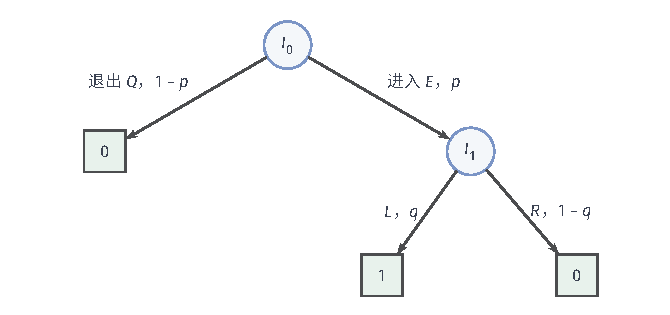
\includegraphics[width=\linewidth]{figures/01-mathematical-preliminaries/05-dynamical-systems-control-decision-and-games/tikz/game-two-stage-self-reach/figure.pdf}
  \caption{同一参与者$i$的两层决策。圆节点是其信息集，方节点中的数值是终局收益。
  第一步以概率$p$进入，第二步在已进入的条件下以概率$q$选$L$；
  因此到达收益为$1$的终局需经过两个本人行动，概率为$pq$。
  本图没有对手或机会节点，是用于区分自身到达概率与局部行动概率的教学构造。}
  \label{fig:game-two-stage-self-reach}
\end{figure}

% Baseline B:972-1018; learning indices normalized
\begin{definition}[反事实价值]
\label{def:game-counterfactual-value}
给定上述联合行为策略及到达权重，参与者\(i\)在信息集\(I\)采取行动\(a\in A(I)\)的
\term{反事实价值}（counterfactual value）定义为
\begin{equation}
  v_i^{\bm{\sigma}}(I,a)
  =
  \sum_{h\in I}
  \pi_{-i}^{\bm{\sigma}}(h)
  \sum_{z\succeq ha}
  \pi^{\bm{\sigma}}(ha,z)u_i(z).
  \label{eq:game-counterfactual-action-value}
\end{equation}
信息集当前策略的反事实价值为
\begin{equation}
  v_i^{\bm{\sigma}}(I)
  =
  \sum_{a\in A(I)}
  \sigma_i(a\mid I)
  v_i^{\bm{\sigma}}(I,a).
  \label{eq:game-counterfactual-value}
\end{equation}

\end{definition}
式~\eqref{eq:game-counterfactual-action-value}保留对手和机会到达\(I\)的权重，
却去掉参与者\(i\)自己在到达\(I\)以前的概率。它在问：假设参与者\(i\)把自己送到
这个信息集，其他方和机会以当前方式到达各节点时，当前行动价值如何。去掉自身到达权重
使一个很少被当前自身策略访问的信息集仍能积累学习信号。

在例~\ref{ex:game-two-stage-self-reach}中，去掉自身前缀概率$p$以后，
$v_i(I_1,L)=1$、$v_i(I_1,R)=0$，当前局部价值为$v_i(I_1)=q$。
选$L$的局部改进量为$1-q$，因而在$p=0$时仍保留信号。
它没有声称当前整局收益已经增加了$1-q$；比较完整替代计划时，
还要补回该计划自己到达$I_1$的概率。

在均衡牌面策略下，参与者2的信息集包含高牌质询与低牌质询两个节点。对参与者2而言，
相应反事实到达权重为
\[
  \frac12 b_H^\star=\frac12,
  \qquad
  \frac12 b_L^\star=\frac16.
\]
若把它们归一化，得到到达信息集后的信念
\[
  \mathbb{P}(H\mid B)=\frac34,\qquad
  \mathbb{P}(L\mid B)=\frac14.
\]
在这组权重下，参与者2选择应对的反事实价值为
$\frac12(-2)+\frac16(2)=-\frac23$，退让的反事实价值为
$(\frac12+\frac16)(-1)=-\frac23$。除以总权重$2/3$后，两项条件期望收益都为$-1$。
局部是否偏好一个行动由同一比例缩放保持，但跨信息集求和必须保留原权重。
后验概率用于该信息集内的条件决策，反事实价值则保留未归一化权重，以便把不同信息集的
局部偏离加回整局收益。两者只差一个到达概率因子，却服务于不同推导。

此处“反事实”不同于第~\ref{chap:causal-inference}章的因果反事实：
前者在既定博弈中去掉本人到达权重，后者固定同一单位的外生背景并替换结构方程。
前者不提供因果识别结论。尤其不能先在每个信息集随意归一化，再把不同位置的条件收益
直接相加充当整局差距。

% Baseline B:1189-1264; learning indices normalized
前两小节采用损失约定，遗憾写成实际损失减替代损失。扩展式博弈沿用收益函数，下面改用
收益约定，把遗憾写成替代收益减当前收益；令损失等于收益的相反数，就能在两种约定之间
转换，正遗憾始终表示偏离更有利。

在第\(k\)轮扩展式博弈中，联合策略记为\(\bm{\sigma}^{(k)}\)。参与者\(i\)在信息集
\(I\)把当前随机行动改成固定行动\(a\)的即时反事实遗憾为
\begin{equation}
  r_i^{(k)}(I,a)
  =
  v_i^{\bm{\sigma}^{(k)}}(I,a)
  -
  v_i^{\bm{\sigma}^{(k)}}(I).
  \label{eq:game-immediate-counterfactual-regret}
\end{equation}
累计量及其正部最大值记为
\[
  R_i^{(K)}(I,a)
  =
  \sum_{k=1}^{K}r_i^{(k)}(I,a),
  \qquad
  R_{i,+}^{(K)}(I)
  =
  \max\left\{0,\max_{a\in A(I)}R_i^{(K)}(I,a)\right\}.
\]

\term{反事实遗憾最小化}（counterfactual regret minimization, CFR）在每个信息集
运行一个局部无遗憾算法\scite{math-zinkevich2007cfr}一次完整树更新包含四步：
固定本轮联合行为策略并遍历历史树，计算各信息集的反事实行动价值；用
式~\eqref{eq:game-immediate-counterfactual-regret}累计每个行动的遗憾；用局部
遗憾匹配生成下一轮策略；同时按本人的到达概率累计平均策略所需的实现权重。这里的
“最小化”是让平均遗憾趋近于零，不是逐轮直接最小化某个静态目标。

典型的\term{遗憾匹配}（regret matching）按正累计遗憾选择下一轮行动：
\begin{equation}
  \sigma_i^{(k+1)}(a\mid I)
  =
  \begin{cases}
    \displaystyle
    \frac{[R_i^{(k)}(I,a)]_+}
         {\sum_b[R_i^{(k)}(I,b)]_+},
      &\sum_b[R_i^{(k)}(I,b)]_+>0,\\[8pt]
    \displaystyle\frac{1}{|A(I)|},
      &\text{否则}.
  \end{cases}
  \label{eq:game-regret-matching}
\end{equation}
所有\(R_i^{(0)}(I,a)\)初始化为零，首轮因此使用均匀分布。

若存在\(\Delta_I\geq0\)，使对每轮\(k=1,\ldots,K\)及任意
\(a,b\in A(I)\)都有
\[
  \left|
    v_i^{\bm{\sigma}^{(k)}}(I,a)
    -
    v_i^{\bm{\sigma}^{(k)}}(I,b)
  \right|
  \leq\Delta_I,
\]
则遗憾匹配满足
\begin{equation}
  R_{i,+}^{(K)}(I)
  \leq
  \Delta_I\sqrt{|A(I)|K}.
  \label{eq:game-local-regret-matching-bound}
\end{equation}
证明可用势函数
\(\Phi^{(k)}=\sum_a[R_i^{(k)}(I,a)]_+^2\)，其中\(\Phi^{(0)}=0\)。
对任意实数\(x,y\)，有
\([x+y]_+^2\leq[x]_+^2+2[x]_+y+y^2\)；
将它用于累计遗憾递推，每轮势函数增量中的交叉项为
\[
  2\sum_a[R_i^{(k-1)}(I,a)]_+r_i^{(k)}(I,a).
\]
当正遗憾和非零时，式~\eqref{eq:game-regret-matching}使它正比于
\(\sum_a\sigma_i^{(k)}(a\mid I)r_i^{(k)}(I,a)=0\)；正遗憾和为零时，
交叉项也不为正。平方增量至多
\(\sum_a(r_i^{(k)}(I,a))^2\leq |A(I)|\Delta_I^2\)。
归纳得到
\(\Phi^{(K)}\leq K|A(I)|\Delta_I^2\)，而每个正累计遗憾的平方不超过
\(\Phi^{(K)}\)，于是得到式~\eqref{eq:game-local-regret-matching-bound}。

% Baseline B:1268-1297; learning indices normalized
用三张牌博弈核对一次参与者2的CFR更新。假设当前策略取
\[
  b_H=b_L=\frac12,\qquad
  \sigma_2(C\mid I_2)=\sigma_2(F\mid I_2)=\frac12.
\]
参与者2到达高牌质询节点和低牌质询节点的反事实权重都为
\[
  \frac12\cdot\frac12=\frac14.
\]
第一个因子来自机会发牌，第二个因子来自参与者1质询。应对
\(C\)时，参与者2在高牌和低牌节点的收益分别为\(-2\)与\(2\)，所以
\[
  v_2(I_2,C)
  =
  \frac14(-2)+\frac14(2)=0.
\]
退让\(F\)时，参与者1在两个节点都得到\(1\)，参与者2因而都得到\(-1\)，所以
\[
  v_2(I_2,F)
  =
  \frac14(-1)+\frac14(-1)=-\frac12.
\]
当前均匀策略的反事实价值为\(-1/4\)，本轮即时遗憾因此为
\[
  r_2(I_2,C)=\frac14,\qquad
  r_2(I_2,F)=-\frac14.
\]
若此前累计遗憾为零，遗憾匹配在下一轮把全部概率放到\(C\)。这个结果只描述一次局部
更新；参与者2更常应对以后，低牌质询会变得不利，参与者1的后续更新又会改变两个节点的
权重。因而不能把首轮纯响应当成收敛策略，也不能从这一个数值步骤推出均衡保证。

\subsubsection{完全回忆下的局部遗憾汇总}
\label{sec:game-perfect-recall-regret}

局部无遗憾尚未回答完整策略能改善多少。证明须把对手与机会的到达权重留在局部量中，
再用同一个替代策略的自身到达概率汇总；完全回忆保证汇总时每条本人决策前缀不含歧义。

% Baseline B:1301-1478; learning indices normalized
整局外部遗憾允许参与者把当前行为策略替换成任意固定行为策略：
\begin{equation}
  R_i^{(K)}
  =
  \max_{\widetilde{\sigma}_i}
  \sum_{k=1}^{K}
  \left[
    u_i(\widetilde{\sigma}_i,\bm{\sigma}_{-i}^{(k)})
    -
    u_i(\bm{\sigma}^{(k)})
  \right].
  \label{eq:game-extensive-external-regret}
\end{equation}
局部反事实遗憾之所以有用，在于它们能够上界这个看似覆盖整棵树的比较。

例~\ref{ex:game-two-stage-self-reach}可以先展示一次拆分。
当前策略为$(p,q)$，完整替代策略为$(\widetilde p,\widetilde q)$时，
\begin{equation}
 \widetilde p\,\widetilde q-pq
 =(\widetilde p-p)q+\widetilde p(\widetilde q-q).
 \label{eq:game-two-stage-deviation}
\end{equation}
第一项只改$I_0$的进入概率，保留当前第二步$q$；
第二项再改$I_1$的行动，乘上的却是替代计划的进入概率$\widetilde p$。
第二步的局部改进先去掉当前自身权重$p$，在完整计划比较中再补回$\widetilde p$，
就能同时处理上游和下游都改变的情况。例如$p=q=0$、$\widetilde p=\widetilde q=1$时，
第一项为零，第二项为$1$，恰好恢复整局收益的增加。
下面把这项拆分沿所有本人信息集重复。

\begin{theorem}[CFR的反事实遗憾分解]
\label{thm:game-cfr-decomposition}
在有限完全回忆扩展式博弈中，
\begin{equation}
  R_i^{(K)}
  \leq
  \sum_{I\in\mathcal{I}_i}
  R_{i,+}^{(K)}(I).
  \label{eq:game-cfr-global-bound}
\end{equation}
\end{theorem}

\begin{proof}
固定替代行为策略\(\widetilde{\sigma}_i\)。证明先在一轮中把整局偏离逐层拆开，再对
轮次求和。为看清拆分发生在哪里，对\(h\in I\)定义当前策略在行动\(a\)后的条件续局
收益
\[
  q_i^{(k)}(h,a)
  =
  \sum_{z\succeq ha}
  \pi^{\bm{\sigma}^{(k)}}(ha,z)u_i(z),
\]
并以\(\widetilde q_i^{(k)}(h,a)\)表示对手和机会仍采用
\(\bm{\sigma}_{-i}^{(k)}\)，而参与者\(i\)从\(ha\)以后采用
\(\widetilde{\sigma}_i\)时的同一数值，即
\[
  \widetilde q_i^{(k)}(h,a)
  =
  \sum_{z\succeq ha}
  \pi^{(\widetilde{\sigma}_i,\bm{\sigma}_{-i}^{(k)})}(ha,z)
  u_i(z).
\]
当前策略从\(h\)出发的续局收益为
\(q_i^{(k)}(h)=\sum_b\sigma_i^{(k)}(b\mid I)q_i^{(k)}(h,b)\)。
在替代收益中加上再减去“只在当前行动改用替代分布、以后仍用当前策略”的收益，逐历史
得到恒等式
\begin{align}
  &\sum_{a\in A(I)}
  \widetilde{\sigma}_i(a\mid I)
  \widetilde q_i^{(k)}(h,a)
  -
  q_i^{(k)}(h)
  \notag\\
  &\quad=
  \sum_{a\in A(I)}
  \widetilde{\sigma}_i(a\mid I)
  \bigl(q_i^{(k)}(h,a)-q_i^{(k)}(h)\bigr)
  \notag\\
  &\qquad\quad+
  \sum_{a\in A(I)}
  \widetilde{\sigma}_i(a\mid I)
  \bigl(
    \widetilde q_i^{(k)}(h,a)-q_i^{(k)}(h,a)
  \bigr).
  \label{eq:game-history-deviation-identity}
\end{align}
第一项只改变当前信息集的行动，第二项只记录当前行动之后继续偏离的收益。

下面把逐历史恒等式汇总到信息集。记
\(\mathcal{C}_i(I,a)\)为采取\(a\)以后、在参与者\(i\)再次行动时首次遇到的本人
信息集集合；若在此之前终止，就没有后继信息集。令
\(\widetilde v_i^{(k)}(I)\)为到达\(I\)的对手与机会权重仍取
\(\pi_{-i}^{\bm{\sigma}^{(k)}}(h)\)，但从\(I\)起参与者\(i\)都采用
\(\widetilde{\sigma}_i\)的反事实价值，并记
\[
  D_i^{(k)}(I)
  =
  \widetilde v_i^{(k)}(I)
  -
  v_i^{\bm{\sigma}^{(k)}}(I),
  \qquad
  L_i^{(k)}(I)
  =
  \sum_a
  \widetilde{\sigma}_i(a\mid I)r_i^{(k)}(I,a).
\]
将式~\eqref{eq:game-history-deviation-identity}乘以
\(\pi_{-i}^{\bm{\sigma}^{(k)}}(h)\)并对\(h\in I\)求和，得到信息集偏离收益恒等式
\begin{equation}
  D_i^{(k)}(I)
  =
  L_i^{(k)}(I)
  +
  \sum_{a\in A(I)}
  \widetilde{\sigma}_i(a\mid I)
  \sum_{I'\in\mathcal{C}_i(I,a)}
  D_i^{(k)}(I').
  \label{eq:game-information-set-deviation-identity}
\end{equation}
这里没有漏掉从\(I\)到\(I'\)之间的概率：这段路径上参与者\(i\)不再行动，对手和
机会的路径概率与\(I\)处已有的权重相乘，正好成为\(I'\)中各历史的
\(\pi_{-i}^{\bm{\sigma}^{(k)}}\)。在遇到下一个本人信息集以前终止的路径上，两种
策略的后续行为相同，故其第二项为零。

完全回忆使本人信息集及边\((I,a)\to I'\)组成一个森林。确切地说，同一信息集
\(I'\)中的所有历史具有相同的本人既往信息集与行动序列，所以每个非根信息集都有唯一的
前驱边；对手或机会的多条历史可以汇入同一个\(I'\)，但这些历史只在
\(\pi_{-i}^{\bm{\sigma}^{(k)}}\)的求和中合并，不会把\(I'\)复制成多个后继。
记\(\widetilde{\pi}_i(I)\)为替代策略沿该唯一本人前缀的行动概率乘积；根信息集的
乘积约定为\(1\)。这正是反事实价值中故意省去的自身到达概率。

现在按一个信息集之后还可能遇到的本人信息集层数归纳。最深信息集没有后继，
式~\eqref{eq:game-information-set-deviation-identity}给出
\(D_i^{(k)}(I)=L_i^{(k)}(I)\)。假设所有深度更小的后继子树都已展开，把它们代回
同一恒等式；由于每个后继只有一个前驱，子树中的每个信息集恰好出现一次，其系数等于
沿唯一前缀的\(\widetilde{\sigma}_i\)行动概率乘积。对森林的所有根求和后便得到
\begin{equation}
  u_i(\widetilde{\sigma}_i,\bm{\sigma}_{-i}^{(k)})
  -
  u_i(\bm{\sigma}^{(k)})
  =
  \sum_{I\in\mathcal{I}_i}
  \widetilde{\pi}_i(I)
  \sum_{a\in A(I)}
  \widetilde{\sigma}_i(a\mid I)r_i^{(k)}(I,a).
  \label{eq:game-global-deviation-identity}
\end{equation}
参与者\(i\)从未行动就终止的历史在两种策略下收益相同，因而不出现在右侧。
式~\eqref{eq:game-global-deviation-identity}明确分开了两类权重：对手与机会的权重
已经包含在\(r_i^{(k)}(I,a)\)中，自身在替代策略下到达\(I\)的权重则是外部系数
\(\widetilde{\pi}_i(I)\)。

替代策略固定后，\(\widetilde{\pi}_i(I)\)和
\(\widetilde{\sigma}_i(a\mid I)\)都不随\(k\)变化。对
式~\eqref{eq:game-global-deviation-identity}求和，并使用
\(0\leq\widetilde{\pi}_i(I)\leq1\)，可得
\begin{align*}
  &\sum_{k=1}^{K}
  \left[
    u_i(\widetilde{\sigma}_i,\bm{\sigma}_{-i}^{(k)})
    -
    u_i(\bm{\sigma}^{(k)})
  \right]\\
  &\quad=
  \sum_I
  \widetilde{\pi}_i(I)
  \sum_a
  \widetilde{\sigma}_i(a\mid I)R_i^{(K)}(I,a)\\
  &\quad\leq
  \sum_I
  \widetilde{\pi}_i(I)
  \max_a R_i^{(K)}(I,a)
  \leq
  \sum_I R_{i,+}^{(K)}(I).
\end{align*}
最后一个不等式也覆盖\(\max_aR_i^{(K)}(I,a)<0\)的情形，因为此时相应正部为零。
右侧与替代策略无关，再对\(\widetilde{\sigma}_i\)取最大，就得到
式~\eqref{eq:game-cfr-global-bound}。
\end{proof}

若缺少完全回忆，同一当前信息集可能汇合不同的本人行动历史。此时局部策略无法知道应该
补回哪条自身到达路径，上述递归可能重复计算或遗漏偏离收益，局部低遗憾便不再自动控制
整局外部遗憾。

结合式~\eqref{eq:game-local-regret-matching-bound}，CFR得到
\begin{equation}
  R_i^{(K)}
  \leq
  \sum_{I\in\mathcal{I}_i}
  \Delta_I\sqrt{|A(I)|K}.
  \label{eq:game-cfr-rate}
\end{equation}
当信息集和行动数固定时，平均正外部遗憾
\([R_i^{(K)}]_+/K=O(K^{-1/2})\)，因而趋于零。

有限树与有界终局收益保证可以为各信息集选择有限的\(\Delta_I\)。
这个界针对遍历完整树、准确计算反事实价值的版本，不依赖末次策略是否单调改善。
若信息集本身改变、遗忘破坏完全回忆，或采样值存在未控制的偏差，
须重新检查分解与局部算法，不能只引用CFR名称。

\subsection{累计保证与平均策略表现}
\label{sec:game-regret-average-guarantees}

累计界要转成均衡误差，还需选对平均方式。一般和博弈保留共同轮次形成的联合分布；
两人零和博弈借助收益的分别线性，把双方的独立平均策略与鞍点差距连接起来。
历史树中还须先平均实现计划，才能恢复合法的行为策略。

\subsubsection{一般和条件下的经验分布保证}
\label{sec:game-empirical-equilibrium}

令第\(k\)轮实际联合行动为\(\bm a^{(k)}\)，经验联合分布为
\[
  \widehat\mu^{(K)}(\bm a)
  =\frac1K\sum_{k=1}^K\mathbb I\{\bm a^{(k)}=\bm a\}.
\]
若第\(i\)方的外部收益遗憾不超过\(\varepsilon_iK\)，则对任意固定行动\(a_i'\)，
直接把累计不等式除以\(K\)便得
\[
  \mathbb E_{\bm A\sim\widehat\mu^{(K)}}[u_i(\bm A)]
  \geq
  \mathbb E_{\bm A\sim\widehat\mu^{(K)}}
     [u_i(a_i',\bm A_{-i})]-\varepsilon_i.
\]
这正是第~\ref{sec:game-correlated-deviations}节的CCE不等式加上误差。
若所有参与者的平均正外部遗憾趋零，有限联合单纯形的紧性保证经验分布的每个极限点
都满足CCE条件，也保证其到CCE集合的距离趋零；未必存在唯一的极限分布。

若每个有向替换\(a_i\to b_i\)的平均内部遗憾至多\(\varepsilon_i\)，那么对任意
映射\(\phi_i:A_i\to A_i\)，有
\[
  \begin{aligned}
    &\mathbb E_{\widehat\mu^{(K)}}[
       u_i(\phi_i(A_i),\bm A_{-i})-u_i(\bm A)]\\
    &\qquad=\frac1K\sum_{a_i\in A_i}R_{a_i\to\phi_i(a_i)}^{(K)}
      \leq |A_i|\varepsilon_i.
  \end{aligned}
\]
这里的\(R\)已改写为收益约定。有限个有向替换控制了所有按建议改动的映射，所以
无内部遗憾给出经验联合分布的CE极限点。若算法直接控制所有映射的交换遗憾，
松弛就是\(\varepsilon_i\)，不必再乘\(|A_i|\)。
这个比较不会把普通外部遗憾算法自动升级为内部遗憾算法。

保留联合相关性确实必要。例如双方行动均为\(A,B\)，以第1方的行动为行、
第2方的行动为列，各格列出双方收益：
\[
  \begin{array}{c|cc}
     &A&B\\ \hline
    A&(2,2)&(0,0)\\
    B&(0,0)&(1,1)
  \end{array}
\]
若实际序列一半轮次为\((A,A)\)、一半为\((B,B)\)，每人平均得\(3/2\)，
改用固定\(A\)只能得\(1\)，改用固定\(B\)只能得\(1/2\)；按建议单独改动也无利。
经验分布是CE。两方边缘平均却都是\((1/2,1/2)\)，将它们独立相乘后，
一方对该边缘选\(A\)得\(1\)、选\(B\)得\(1/2\)，混合只得\(3/4\)，所以平均边缘
的乘积不是Nash均衡。

这些是对已记录联合序列的代数结论。若算法控制的是期望损失遗憾，而这里使用抽样行动，
还须估计两者之间的随机误差；每轮独立抽样也不消除跨轮共同变化产生的相关性。

\subsubsection{零和条件下的平均策略保证}
\label{sec:game-zero-sum-average}

矩阵博弈中，\(\bar{\bm x}^{(K)}=K^{-1}\sum_k\bm x^{(k)}\)与
\(\bar{\bm y}^{(K)}=K^{-1}\sum_k\bm y^{(k)}\)仍在各自单纯形内。
固定一方策略时，双线性收益可把另一方的平均移进或移出求和。
历史树中的行为概率却在同一条路径上相乘，逐信息集算术平均一般没有这项性质。

仍用例~\ref{ex:game-two-stage-self-reach}的小树，考虑表~\ref{tab:game-two-stage-average}中的两轮策略。
先等概率抽取一轮，再执行该轮的完整策略，终局$L$的概率为$(1+0)/2=1/2$。
若分别平均两个节点的行动概率，就会得到$\bar p=\bar q=1/2$，
从而把终局$L$的概率改成$\bar p\bar q=1/4$。
错误来自第二轮的$q^{(2)}=0$：这一轮始终退出，第二步怎样选择本来都没有作用，
普通平均却把这个未执行的安排与第一轮同等计入。

\begin{table}[htbp]
  \centering
  \setlength{\tabcolsep}{4pt}
  \begin{tabular}{cccc}
    \toprule
    轮次$k$ & $p^{(k)}$ & $q^{(k)}$ & 终局$L$概率\\
    \midrule
    $1$ & $1$ & $1$ & $1$\\
    $2$ & $0$ & $0$ & $0$\\
    \bottomrule
  \end{tabular}
  \caption{两层小树中的两轮完整策略。$p^{(k)}$表示进入概率，$q^{(k)}$表示进入后选$L$的概率，
  最后一列为$p^{(k)}q^{(k)}$。第二轮不进入，故该轮第二步的安排不影响终局分布。
  这些数值只用于比较策略平均方式，不表示CFR必然产生这样的两轮轨迹。}
  \label{tab:game-two-stage-average}
\end{table}

按本人到达权重平均第二步，则
\[
 \bar q=
 \frac{p^{(1)}q^{(1)}+p^{(2)}q^{(2)}}{p^{(1)}+p^{(2)}}=1,
 \qquad \bar p=\frac12,
\]
使$\bar p\bar q=1/2$，恢复完整策略混合的终局概率。
若两轮都不进入，分母为零，此时任意$\bar q$都与$\bar p=0$组合成相同终局分布。
这个计算依赖$I_1$有唯一本人前缀$I_0\xrightarrow{E}I_1$；
完全回忆把这一性质推广到一般信息集，才能逐层恢复平均后的实现权重。

% Baseline B:1482-1608; learning indices normalized
行为策略不能在每个信息集直接做普通算术平均。某轮中一个信息集若几乎不会被参与者自己
到达，该处局部概率不应与频繁到达轮次具有同样权重。完全回忆保证同一信息集
\(I\)中的历史具有同一条本人行动前缀，因而
\(\pi_i^{\bm{\sigma}^{(k)}}(I)\)定义为这条前缀上的本人行动概率乘积，与选取
哪个\(h\in I\)无关。记第\(k\)轮在本人序列\((I,a)\)上的实现权重为
\[
  x_i^{(k)}(I,a)
  =
  \pi_i^{\bm{\sigma}^{(k)}}(I)
  \sigma_i^{(k)}(a\mid I),
\]
并令
\(\overline{x}_i^{(K)}(I,a)=K^{-1}\sum_k x_i^{(k)}(I,a)\)以及
\(\overline{x}_i^{(K)}(I)=K^{-1}\sum_k
\pi_i^{\bm{\sigma}^{(k)}}(I)\)。CFR使用
\begin{equation}
  \overline{\sigma}_i^{(K)}(a\mid I)
  =
  \frac{
    \sum_{k=1}^{K}
    \pi_i^{\bm{\sigma}^{(k)}}(I)
    \sigma_i^{(k)}(a\mid I)
  }{
    \sum_{k=1}^{K}
    \pi_i^{\bm{\sigma}^{(k)}}(I)
  },
  \label{eq:game-cfr-average-strategy}
\end{equation}
其中分母为零时可以任意指定。式~\eqref{eq:game-cfr-average-strategy}等价于
\[
  \overline{\sigma}_i^{(K)}(a\mid I)
  =
  \frac{\overline{x}_i^{(K)}(I,a)}{\overline{x}_i^{(K)}(I)}.
\]

这个权重不是经验修正，而是实现计划平均所要求的条件概率。根本人序列的实现权重为
\(1\)。若\(I\)的唯一本人前驱序列终止于\((J,b)\)，则每一轮都有
\(\pi_i^{\bm{\sigma}^{(k)}}(I)=x_i^{(k)}(J,b)\)，对轮次平均后仍有
\(\overline{x}_i^{(K)}(I)=\overline{x}_i^{(K)}(J,b)\)。从根序列归纳，并在每个信息集应用
上面的条件概率公式，得到
\begin{equation}
  \pi_i^{\overline{\sigma}_i^{(K)}}(I)
  \overline{\sigma}_i^{(K)}(a\mid I)
  =
  \overline{x}_i^{(K)}(I,a)
  =
  \frac{1}{K}\sum_{k=1}^{K}x_i^{(k)}(I,a).
  \label{eq:game-average-realization-plan}
\end{equation}
因此，加权平均行为策略实现的正是各轮本人实现计划的算术平均。分母为零意味着所有轮次
到达该本人序列的概率都为零，此处怎样指定局部策略都不改变平均实现计划。

在两人零和博弈中，若双方累计外部遗憾分别不超过
\(\varepsilon_1K\)与\(\varepsilon_2K\)，则平均策略满足
\begin{equation}
  \max_{\sigma_1}
  u_1(\sigma_1,\overline{\sigma}_2^{(K)})
  -
  \min_{\sigma_2}
  u_1(\overline{\sigma}_1^{(K)},\sigma_2)
  \leq
  \varepsilon_1+\varepsilon_2.
  \label{eq:game-average-exploitability}
\end{equation}
下面补出这个界。记第\(k\)轮第1位参与者的收益为
\(u_1(\sigma_1^{(k)},\sigma_2^{(k)})\)，并令
\[
  \widehat u^{(K)}
  =
  \frac{1}{K}
  \sum_{k=1}^{K}
  u_1(\sigma_1^{(k)},\sigma_2^{(k)}).
\]
终止历史\(z\)的概率可以写成机会概率与双方实现权重之积，所以期望收益对双方实现计划
分别线性。结合式~\eqref{eq:game-average-realization-plan}，对任意固定策略
\(\sigma_1,\sigma_2\)有
\begin{align}
  \frac{1}{K}\sum_{k=1}^{K}
  u_1(\sigma_1,\sigma_2^{(k)})
  &=
  u_1(\sigma_1,\overline{\sigma}_2^{(K)}),
  \notag\\
  \frac{1}{K}\sum_{k=1}^{K}
  u_1(\sigma_1^{(k)},\sigma_2)
  &=
  u_1(\overline{\sigma}_1^{(K)},\sigma_2).
  \label{eq:game-average-payoff-linearity}
\end{align}

第1位参与者的外部遗憾界除以\(K\)，再用第一条等式，得到
\begin{equation}
  \max_{\sigma_1}
  u_1(\sigma_1,\overline{\sigma}_2^{(K)})
  -
  \widehat u^{(K)}
  \leq
  \varepsilon_1.
  \label{eq:game-row-average-regret}
\end{equation}
第2位参与者的收益为\(u_2=-u_1\)。把其外部遗憾界同样除以\(K\)，并用
式~\eqref{eq:game-average-payoff-linearity}的第二条等式，得到
\begin{equation}
  \widehat u^{(K)}
  -
  \min_{\sigma_2}
  u_1(\overline{\sigma}_1^{(K)},\sigma_2)
  \leq
  \varepsilon_2.
  \label{eq:game-column-average-regret}
\end{equation}
将式~\eqref{eq:game-row-average-regret}与
\eqref{eq:game-column-average-regret}相加，经验对局收益
\(\widehat u^{(K)}\)消去，正好得到
式~\eqref{eq:game-average-exploitability}。若博弈值为\(v^\star\)，其左侧还可写成
\[
  \left[
    \max_{\sigma_1}u_1(\sigma_1,\overline{\sigma}_2^{(K)})-v^\star
  \right]
  +
  \left[
    v^\star-\min_{\sigma_2}u_1(\overline{\sigma}_1^{(K)},\sigma_2)
  \right].
\]
两项分别衡量第2位和第1位参与者的平均策略可被最佳响应利用多少，且都非负；因此该和是
双方平均策略的零和鞍点间隙。本章把这个和称为\term{联合可利用度}
（joint exploitability）；若采用两项平均的口径，数值还需除以\(2\)。间隙为零时，
两者构成极小极大策略对。

一个两步单方例能看清权重的作用：首步以概率\(p\)继续，继续后以概率\(q\)选\(a\)。
两轮采用\((p^{(1)},q^{(1)})=(1,1)\)、\((p^{(2)},q^{(2)})=(0,0)\)。
两轮平均到达终局\(a\)的概率为\(1/2\)。若分别算术平均，得到\(p=q=1/2\)，
终局概率变成\(1/4\)，并未实现原平均。按自身到达概率加权则得到
\(\bar p=1/2,\bar q=(1\cdot1+0\cdot0)/(1+0)=1\)，恢复正确的\(1/2\)。
三张牌中每人只行动一次，各自信息集没有本人先前行动，权重恰好都为\(1\)；
因此这个特例可以直接平均\(b_H,b_L,c\)，不能据此推广到多步决策。

式~\eqref{eq:game-average-exploitability}保证的是两人零和博弈的平均策略，而非末项。
有限完全回忆时，合法平均和极小极大结构共同支持这项结论；一般和的联合经验分布
结论已在上一小节单独建立。

% Baseline B:1637-1664; learning indices normalized
末次策略还可能持续循环。采样CFR若只访问部分历史，还要用第
\ref{chap:stochastic-processes-and-approximation}章的无偏估计、方差和集中工具控制
采样误差，不能把完整树上的确定性分解直接当作有限样本保证。

回到三张牌例子，参与者2的信息集使用高牌质询权重\(1/2\)和低牌质询权重\(1/6\)
计算局部应对遗憾。若算法长期发现应对比退让更好，就提高\(C\)的概率；这一变化又会
降低低牌质询的收益，使参与者1减少虚张声势。双方局部更新相互改变下一轮价值，CFR保证
累计偏离受控，却不要求这两个概率逐轮单调走向\(1/3\)。

把平均遗憾转成均衡结论时，还要保留产生平均的联合样本。
表~\ref{tab:game-regret-comparison-conclusions}比较两种偏离：固定行动只提出一个
事前替代选择，内部替换可以对某种已采取行动单独修改，因此后者需要控制更多比较。
这里的保证针对经验联合分布或相应的平均策略，不对最后一轮作同样承诺。

\begin{table*}[htbp]
  \centering
  \begin{tabularx}{\linewidth}{lXXX}
    \toprule
    偏离比较 & 允许怎样改变 & 一般和下的平均结论 & 两人零和的补充\\
    \midrule
    外部遗憾 & 所有轮次统一改用一个固定行动 & 经验联合分布的粗相关偏离收益小 & 双方平均策略的鞍点差距小\\
    内部遗憾 & 将某种已选行动统一换成另一行动 & 经验联合分布的相关偏离收益小 & 仍需按具体信息结构恢复策略\\
    \bottomrule
  \end{tabularx}
  \caption{遗憾的比较类与平均结论。表中要求每位参与者都控制相应的平均遗憾；
  扩展式博弈的平均行为策略还须使用自身到达权重。末次策略收敛不由这些平均结论推出。}
  \label{tab:game-regret-comparison-conclusions}
\end{table*}

\section{本章小结}
\label{sec:game-theory-and-multi-agent-decision-summary}

多方选择使行动的后果取决于联合策略。信息集先限制每人能够实施的完整计划，
到达概率再把这些计划变成各方整局价值。完全回忆保证混合计划与行为策略的实现等价，
也为后面的局部遗憾分解提供唯一本人前缀。三张牌博弈中，是否看得见隐藏牌会改变
合法策略，不只是改变收益估计。

固定其他策略后可求最佳响应，相互响应形成Nash条件。有限混合均衡的存在由
Sperner、Brouwer、闭图近似选择和Kakutani的证明链保证，不意味着唯一、容易计算或
能够被任意学习过程找到。零和极小极大把双方保证写成一对线性规划，三张牌的
\(2/3\)由原对偶可行证书共同确认。共同建议则改变偏离时可用的信息，得到CE与CCE
各自的约束；它们不能与独立混合Nash无条件互换。

给定更新规则以后，才能检验其不动点和稳定性。双加热器的一步响应误差可以收缩，
但这与局内温差在固定反馈下的衰减是两套计算。匹配硬币同时响应会形成四周期，
同时离散梯度在中心附近会放大扰动，连续梯度或复制动态还可能沿闭轨道运行。
ESS另行检验少量新策略的入侵，不能用名称中的“稳定”代替指定更新的分析。

没有末项收敛时，累计比较仍有意义。投影次梯度用固定比较点的距离递推给出
\(O(\sqrt K)\)外部遗憾；CFR保留对手与机会的反事实权重，再沿完全回忆的信息集
森林汇总局部偏离。一般和无外部或内部遗憾控制相应的经验CCE或CE误差，
两人零和的双方遗憾则控制合法平均策略的联合可利用度。平均行为策略须由平均实现
计划恢复，不能逐位置任意平均，也不能把完整树的确定性证明当作采样保证。

合作价值回答另一类问题。Shapley值在联盟价值已定义后按加入顺序平均边际贡献，
并由四项公理唯一刻画；它既不保证成员不退出，也不把预测归因变成因果贡献。
核心检验联盟阻挡，Pareto条件排除共同改善，Nash乘积协商在声明的紧凸可行域、
共同严格增益和分歧点下选择唯一收益向量。公平分配、无获利偏离、动态稳定、
末项收敛和无遗憾各有比较对象与条件，任何一项都不能仅凭另一项的名称推出。
下一章将把这些保证放回后续机器学习任务，比较它们各自回答的问题。
